\documentclass[a4paper,12pt]{report}

% Page Layout
\usepackage{geometry}
\geometry{
  a4paper,
  left=20mm,
  right=20mm,
  bottom=15mm,
  top=15mm
}
\usepackage{Archivo}
\usepackage[T1]{fontenc}
\sffamily

\usepackage{subcaption}
\usepackage{graphicx, wrapfig, xcolor, multicol}
\usepackage{tikz, pgfplots}
\usepgflibrary{shadings}
\usetikzlibrary{positioning, shapes.geometric, fit}
\pgfplotsset{compat=1.18}
\usepackage{amsmath, amssymb, amsthm, mathtools}
\usepackage[most]{tcolorbox}
\graphicspath{{images/}}

\linespread{1.3}
\usepackage{url}
\urlstyle{same}
\usepackage{hyperref}
\hypersetup{
    colorlinks=true,
    linkcolor=blue,
    filecolor=magenta,
    urlcolor=cyan,
  }


% ------------------------------------------------------------------------------------------------------------------
\begin{document}
\thispagestyle{empty}
\vspace*{4mm}
\begin{center}
  {\Large
  A\\
  Report on}\\[3mm]
  \begin{tcolorbox}[colback=blue!20, colframe=blue!20]
    \centering
  {\bfseries \Large  A Workshop on LaTex Tutorial and \\[3mm]
    Advanced Techniques for Beginners and Beyond}
  \end{tcolorbox}
\vspace{7mm}
    Organized by: \textcolor{blue!50!cyan}{Central Department of Mathematics, IoST, Tribhuvan University, Kathmandu,Nepal}

    \vspace{7mm}
    \begin{figure}[h!]
      \centering
      
\includegraphics[width=3.5cm, height=4cm]{tulogo1.png}
    \end{figure}

    \vspace{17mm}

    {\bfseries \Large Submitted to} \\[5mm]

    \textbf{NHEP, TU-PSU}\\
    Office of the Planning Directorate,\\
    Tribhuvan University, Kirtipur Kathmandu.\\[10mm]

     {\bfseries Submitted by} \\[1mm]
     \textcolor{blue!60!cyan}{Central Department of Mathematics, IoST, TU}

     \vspace{10mm}
     May, 2024
     \vspace{3mm}
     \begin{tcolorbox}[colback=blue!20, colframe=blue!20]
       \Large \centering
       \textbf{Venue}: \hspace{2mm} Central Department of Mathematics, \\
       Kritipur, IoST, TU
     \end{tcolorbox}

\end{center}
\clearpage

\vspace*{5mm}
{\bfseries \Large Background Information}\\[4mm]
The Central Department of Mathematics, Institute of Science and Technology , Tribhuvan University, Kathmandu Nepal organized a Workshop on LaTex Tutorial and Advanced Techniques for Beginners and Beyond. It was a 3-day workshop which ran from May 2, 2024 Thursday to May 4, 2024 Saturday. Thursday and Saturday were physical sessions which took place inside the Central Department of Mathematics, TU, Kritipur, Nepal. Friday was online session which took place via zoom meeting.
\vspace{5mm}

\begin{figure}[h!]
  \centering
  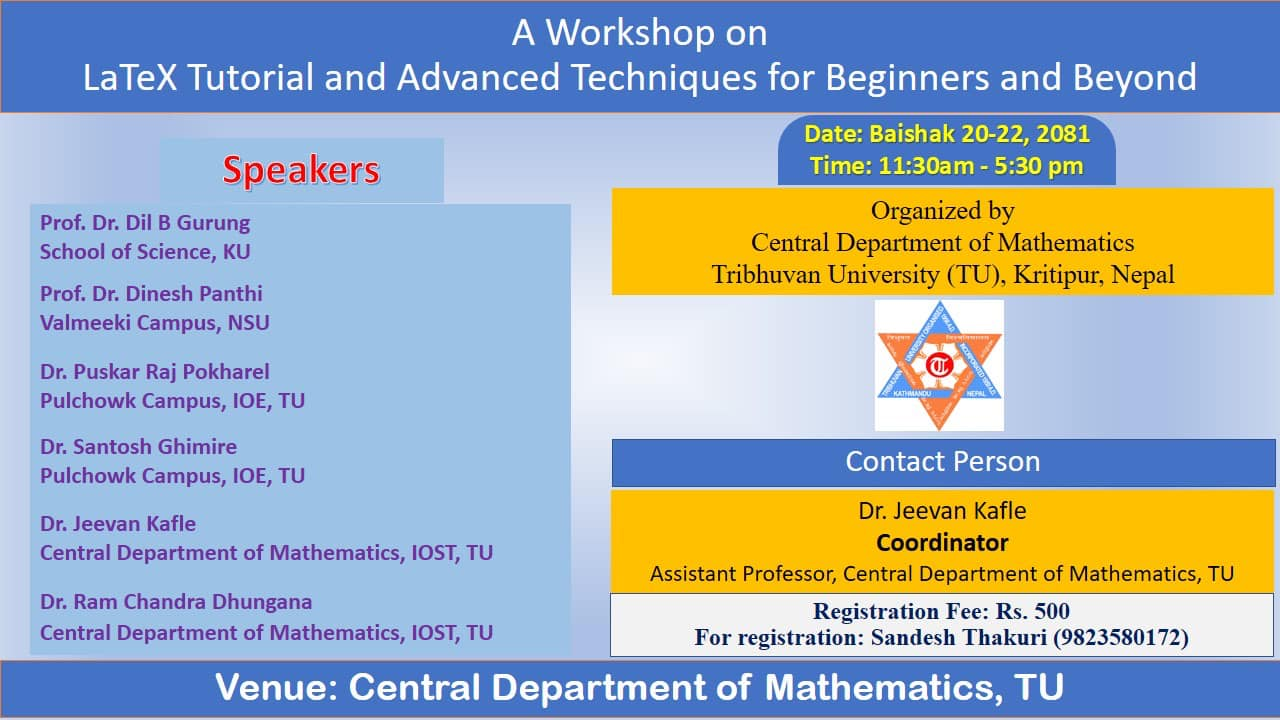
\includegraphics[scale=0.33]{flyer.jpg}
\end{figure}
\vspace{9mm}

\noindent
The chairman of the workshop was the HoD Prof. Dr. \textbf{Chet Raj Bhatta}. The workshop was coordinated by \textbf{Dr. Jeevan Kafle} who is a leading figure in mathematics and a faculty of the Central Department of Mathematics, TU whose area of research is modelling in natural and applied sciences. The organizing team consisted of \textbf{CDM Student Council} who took all the management responsibilities of the workshop under the leadership of the President of the Council \textbf{Mr. Sandesh Thakuri}. Other members of the team were:
\begin{itemize}
\item Sec. Manoj KC
\item VP. Biddha Pokhrel
\item Treasurer. Dhakaram Regmi
\end{itemize}

\noindent
The Chief-Guest of the workshop was the Director of Research Directorate, TU Prof. Dr. \textbf{Ishwar Koirala}.
\clearpage

\noindent
{\bfseries \Large Experts and Resource person}\\[3mm]
Six experts from the three universities of Nepal came to train during the workshop. The list of experts was as follows:

\begin{table}[h!]
\centering
  \begin{tcolorbox}[colframe=blue!52, colback=white, width=\linewidth]
\centering  \footnotesize
\begin{tabular}{l||c}

    1. Prof. Dr. Dil Bahadur Gurung &
    \textit{School of Science, Dhulikhel, Kathmandu University}\\
    \\
    2. Dr. Dinesh Panthi &
    \textit{Valmeeki Campus, Kathmandu, Nepal Sanskrit University}\\
    \\
    3. Dr. Puskar Raj Pokharel &
    \textit{Pulchowk Campus, IoE, Tribhuvan University}\\
    \\
    4. Dr. Santosh Ghimire&
    \textit{Pulchowk Campus, IoE, Tribhuvan University}\\
    \\
    5. Dr. Jeevan Kafle &
    \textit{Central Department of Mathematics, TU}\\
    \\
    6. Dr. Ram Chandra Dhungana &
    \textit{Central Department of Mathematics, TU}\\
    \end{tabular}
  \end{tcolorbox}
\end{table}

\noindent
The guests of the workshop on its first day were the:
\begin{itemize}
\item Vice-President of Nepal Mathematical Society Assoc. Dr. Shree Ram Khadka
\item President of CDM Alumni Association Nepal Prof. Dr. Gyan Bahadur Thapa.
\item Assistant Dean of IoE, TU, Dr. Puskar Raj Pokharel
\end{itemize}

\noindent
This workshop was attended by around \textbf{31 participants} who were the research students from the central department of mathematics, TU and faculties from various campuses of TU. The number of the participants in this workshop was made limited due to lab-based model of the workshop and the technological demands of the workshop. Note books for the workshop was sponsored by the \textbf{Sukunda Pustak Bhawan}.

\begin{figure}[hb!]
  \centering
  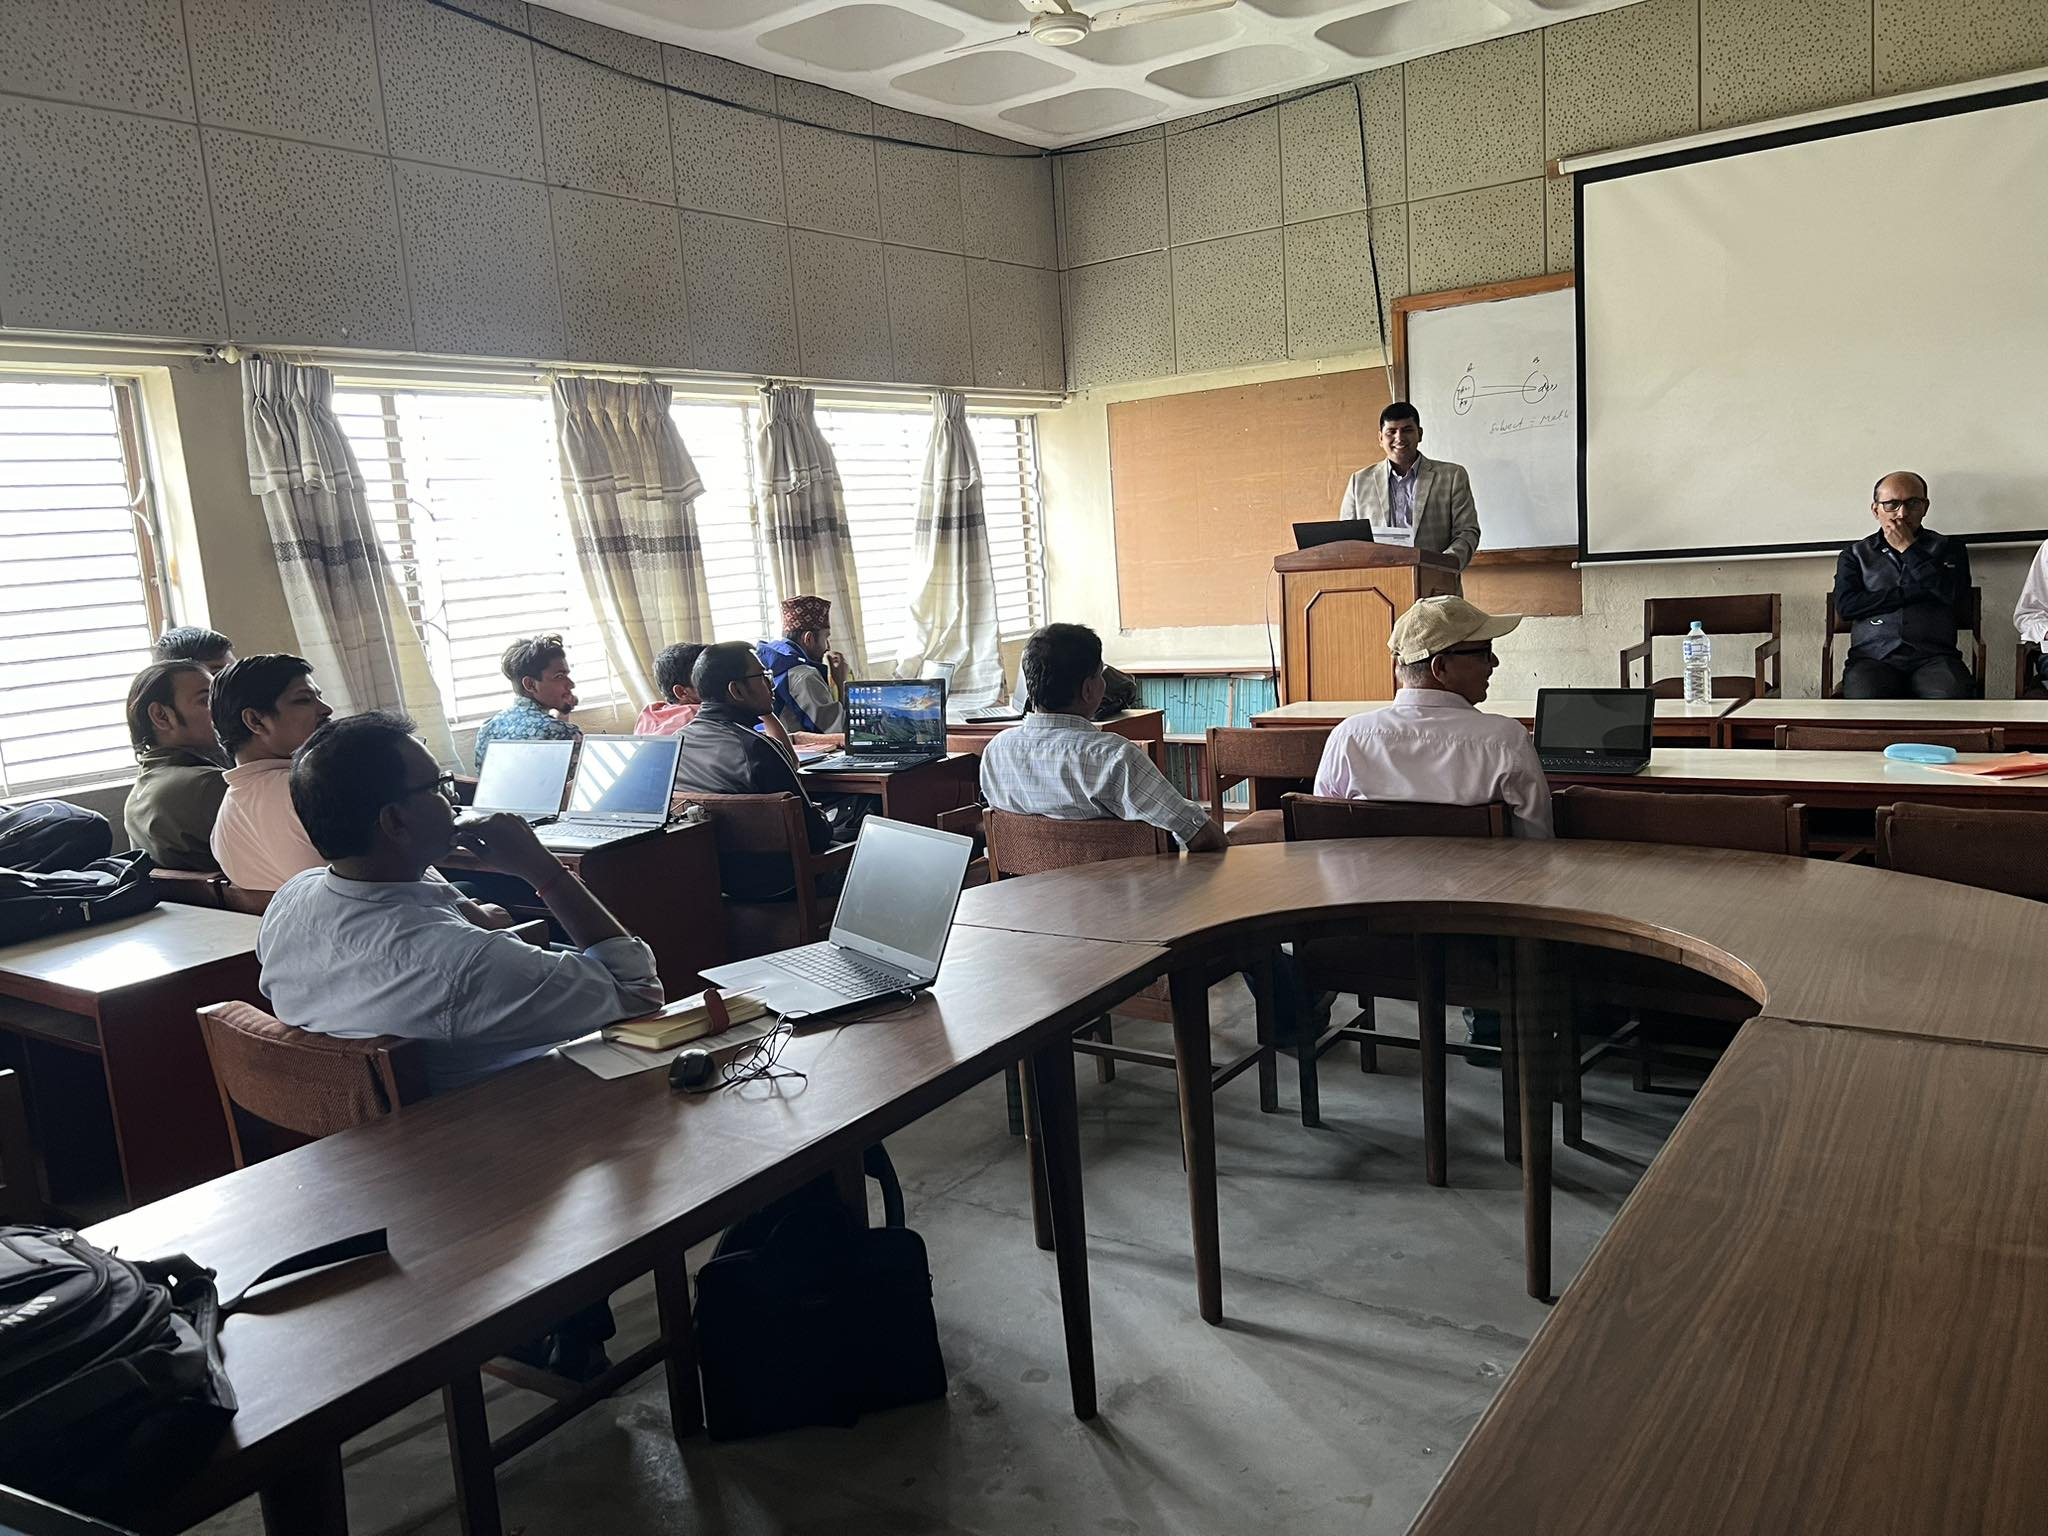
\includegraphics[width=14cm, height=7.5cm]{jeevansir.jpg}
  \caption{Dr. Kafle inaugurating the workshop}
\end{figure}
\clearpage


{\Large \textbf{Objectives}}\\

This workshop was organized with the following objectives:
\begin{itemize}
\item Facilitate Phd Scholars, Mphil Scholars, Master Scholars with training on latex.
\item Make the research writings (thesis and articles) latex oriented.
\end{itemize}

\vspace{15mm}
{\Large \textbf{Program Schedule}}\\
\begin{figure}[h!]
  \centering
  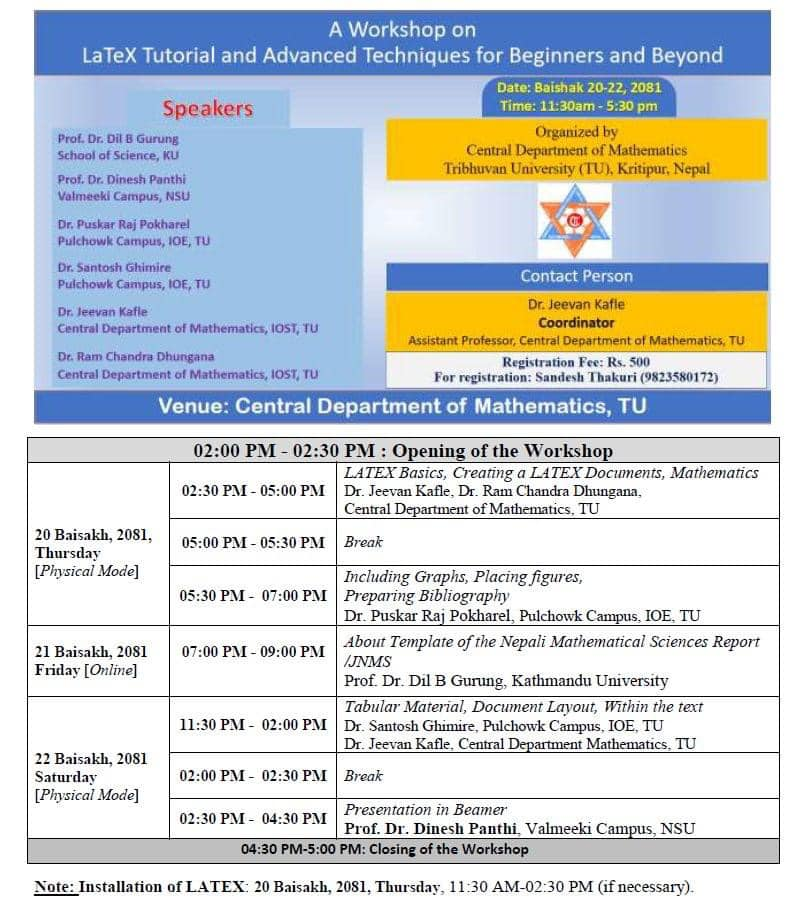
\includegraphics[width=17cm, height=18cm]{schedule.jpg}
\end{figure}
\clearpage

\vspace*{1cm}
{\Large \textbf{Methodology}}\\[5mm]
The methods applied to make this workshop happen were both online method and physical method.
\vspace{2mm}
\begin{itemize}
\item \textbf{Online}\\[2mm]
  The online method was one of the demand of the workshop. For this there was an online session which was done via \textbf{zoom-meeting}. The first reason for this was that the expert Dr. \textbf{Dil Bahadur Gurung} was at Kathmandu University, Dhulikhel another district from the venue of the workshop. He could not manage to be physically because of the distance and time schedule. The nature of this session demanded online session because the tools used in this session was websites and web-links to the journals and their templates rather than the slides. This session was knowledge intensive rather than practice intensive. Also the information about the scientific journals and the article writing was more than the scope of latex. It was a general thing every researcher should know despite the formulation of its template not being in latex. So this session needed to be open to all the researchers and this was possible only through an online session. \vspace{2cm}

\item \textbf{Physical}\\[2mm]
  The physical method was the primary demand of the workshop as any workshop of such nature is incomplete without it. This workshop required intensive practice and training in presence of experts. This is possible only in a lab-based room with experts and projectors, boards and illustrations. The physical sessions were done in the \textbf{seminar hall} of the department which was equipped with a projector, screen and a board. Participants came with their own \textbf{laptops} and multi-plugs were managed by the department of the proper charging of the laptops during the workshop. The experts first illustrated the work in the screen via projector then the participants were guided to practice. Once the participants were confident about the concept the expert moved on to the next concept. This process was carried out throughout the sessions.
\end{itemize}
\clearpage

{\bfseries \Large Inaugural Session}\\[3mm]
The inauguration session was short and formal. Dr. \textbf{Kafle} was at mike. It was from 2pm to 2:30pm. Before 2pm, participants were facilitated with latex installation and all the necessary software installation for the workshop by Dr. Dhungana. And they were provided a note book, a pen and the program schedule after registration by Mr. Sandesh Thakuri.\\[2mm]

\noindent
The \textbf{Chief-Guest} Dr. Koirala spoke about how crucial the \textit{latex} is to the science researchers. It is the de facto standard for the research articles in the scientific journals and publications. Latex format is compulsory in most scientific journals and publications. He said he learned it during his time in an Engineering Collage and consistent practice is the need for learning the latex program.\\
He being the director at Research Directorate at TU talked about the research funding and grants provided by TU for the different types of researchers both at University level and National level. The range of grant provided are from 20 thousands to 1 core. The quotas for the grant are 5-8 for the PhD Professors, several for Mphil students, 50 for master students  and so on. But the rules are strict, the research done must aid in policy making of the Neplease Goverment.

\vspace{5mm}
\begin{figure}[h!]
  \centering
  \begin{subfigure}{0.52\textwidth}
    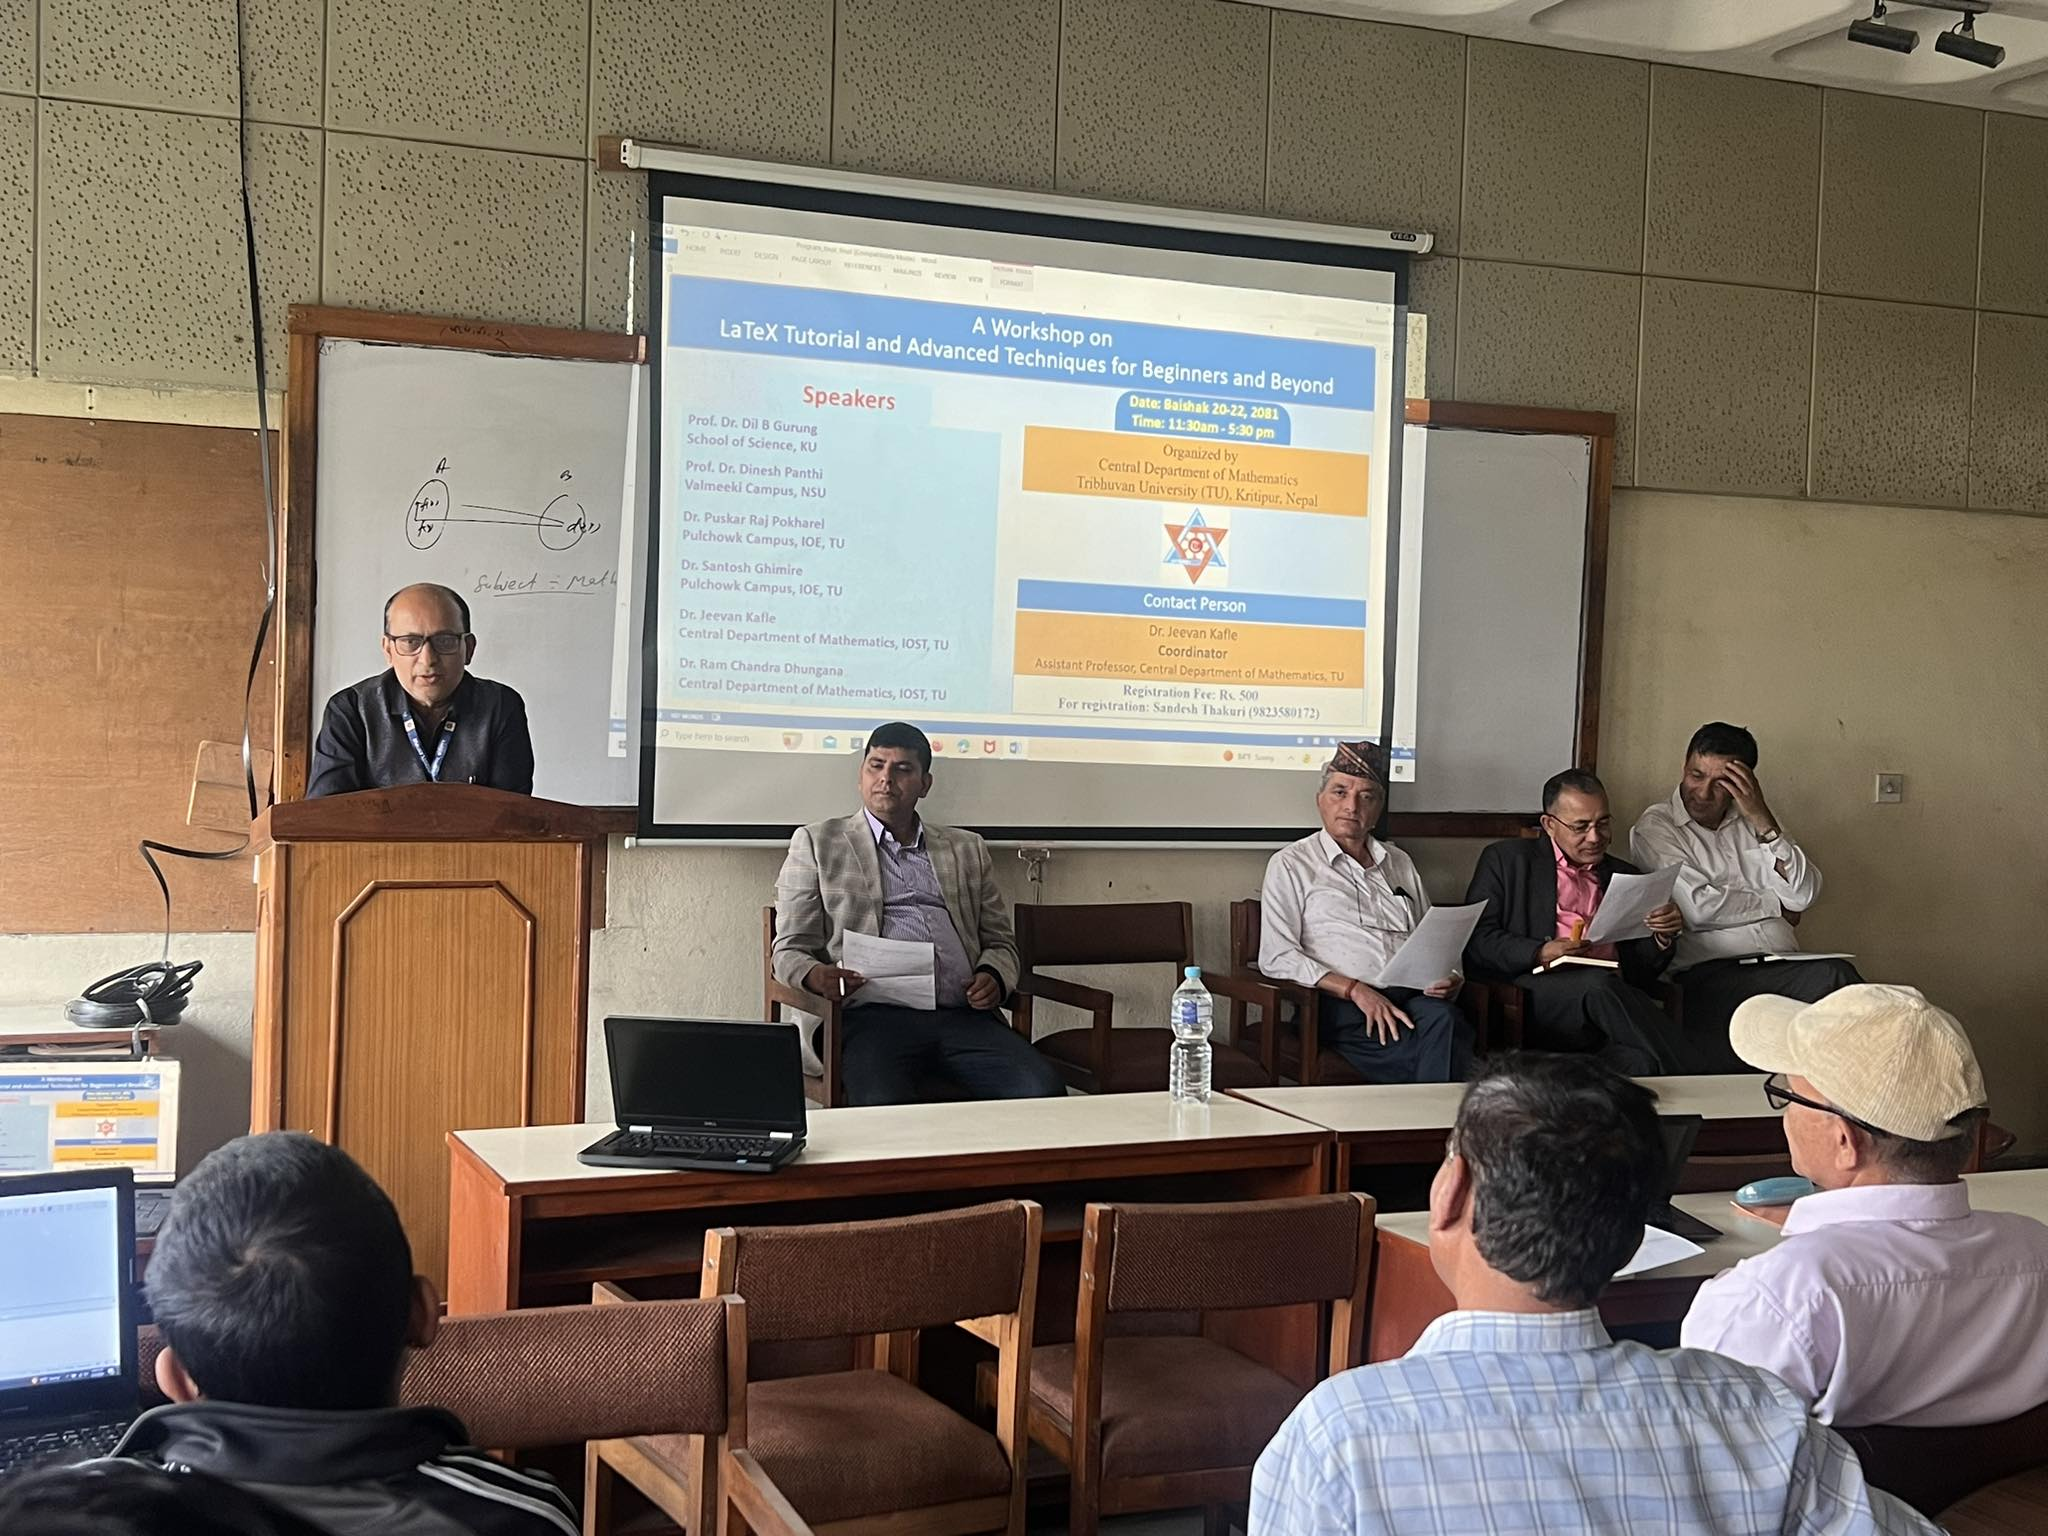
\includegraphics[height=7cm, width=\textwidth]{cheifguest.jpg}
    \caption{Chief Guest Dr. Ishwar Koirala}
    \label{fig:first}
\end{subfigure}
\hfill
\begin{subfigure}{0.42\textwidth}
    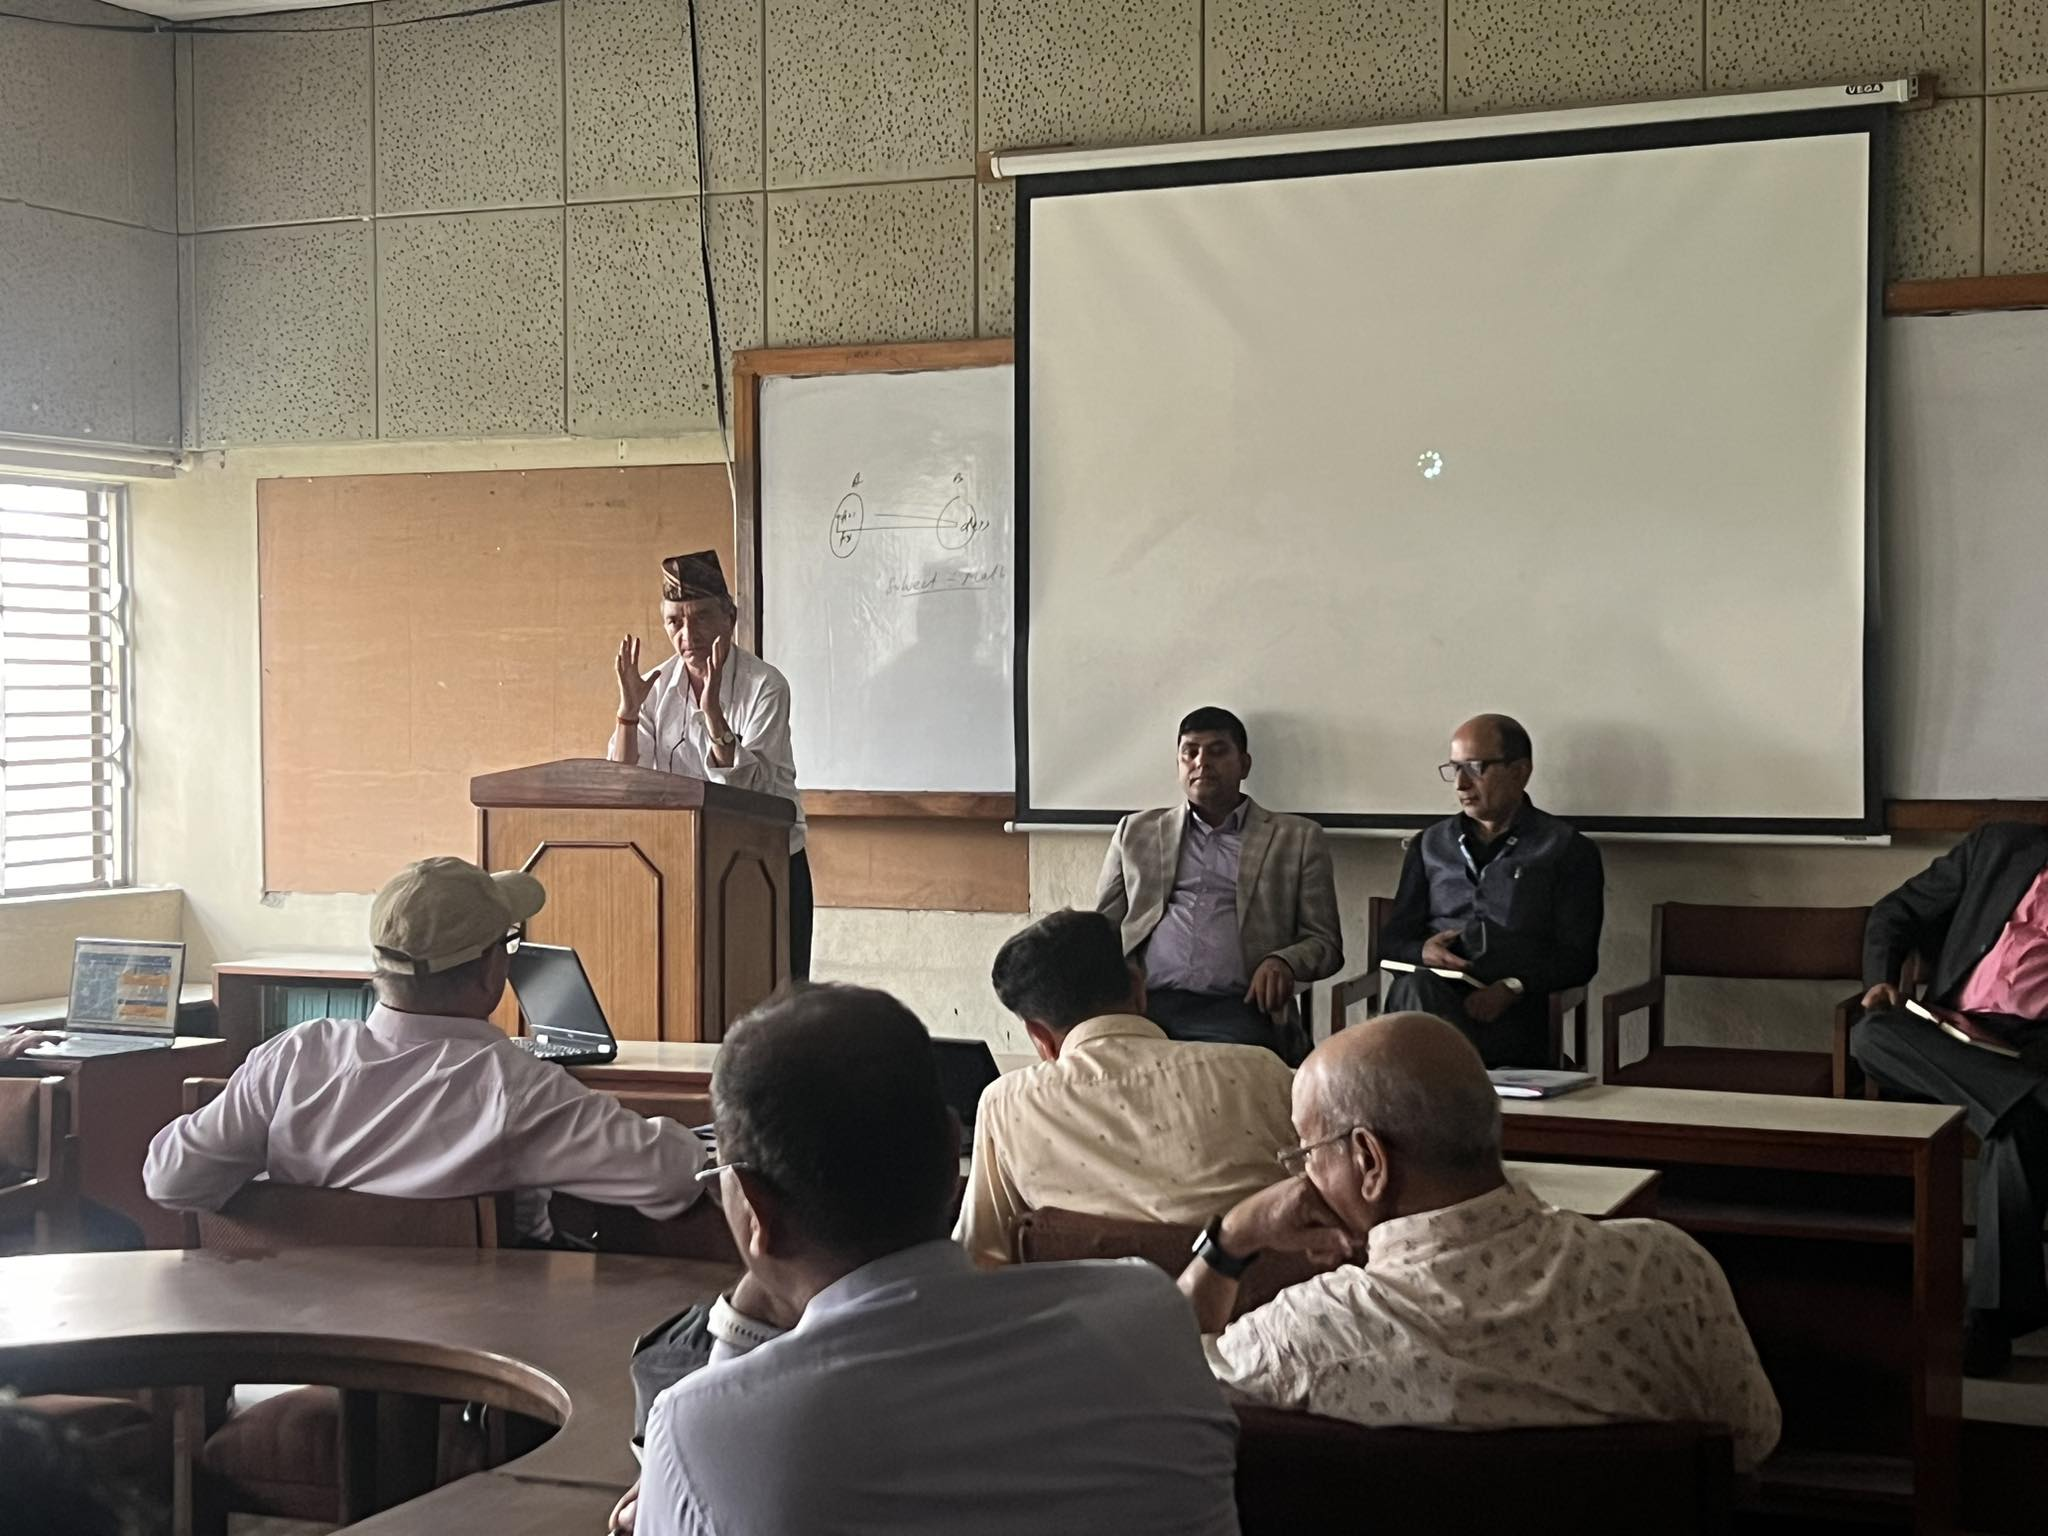
\includegraphics[height=7cm, width=\textwidth]{chet.jpg}
    \caption{Chairman Dr. Bhatta}
    \label{fig:second}
\end{subfigure}
\end{figure}

\vspace{5mm}
\noindent
The Chairman of the workshop HoD Prof. Dr. {Chet Raj Bhatta} praised and thanked the coordinator of the workshop Dr. Kafle for his dedication and hard work in making this workshop happen. He also thanked the whole organizing team for their support and hard work. He welcomed all the guests and participants and gave his best wishes for the success of the workshop. He asked every participants to make the best out of this workshop and learn as much as possible and share their knowledge to others as well after the completion of the workshop.
\clearpage


\vspace*{5mm}
\begin{figure}[h!]
\centering
\begin{subfigure}{0.45\textwidth}
    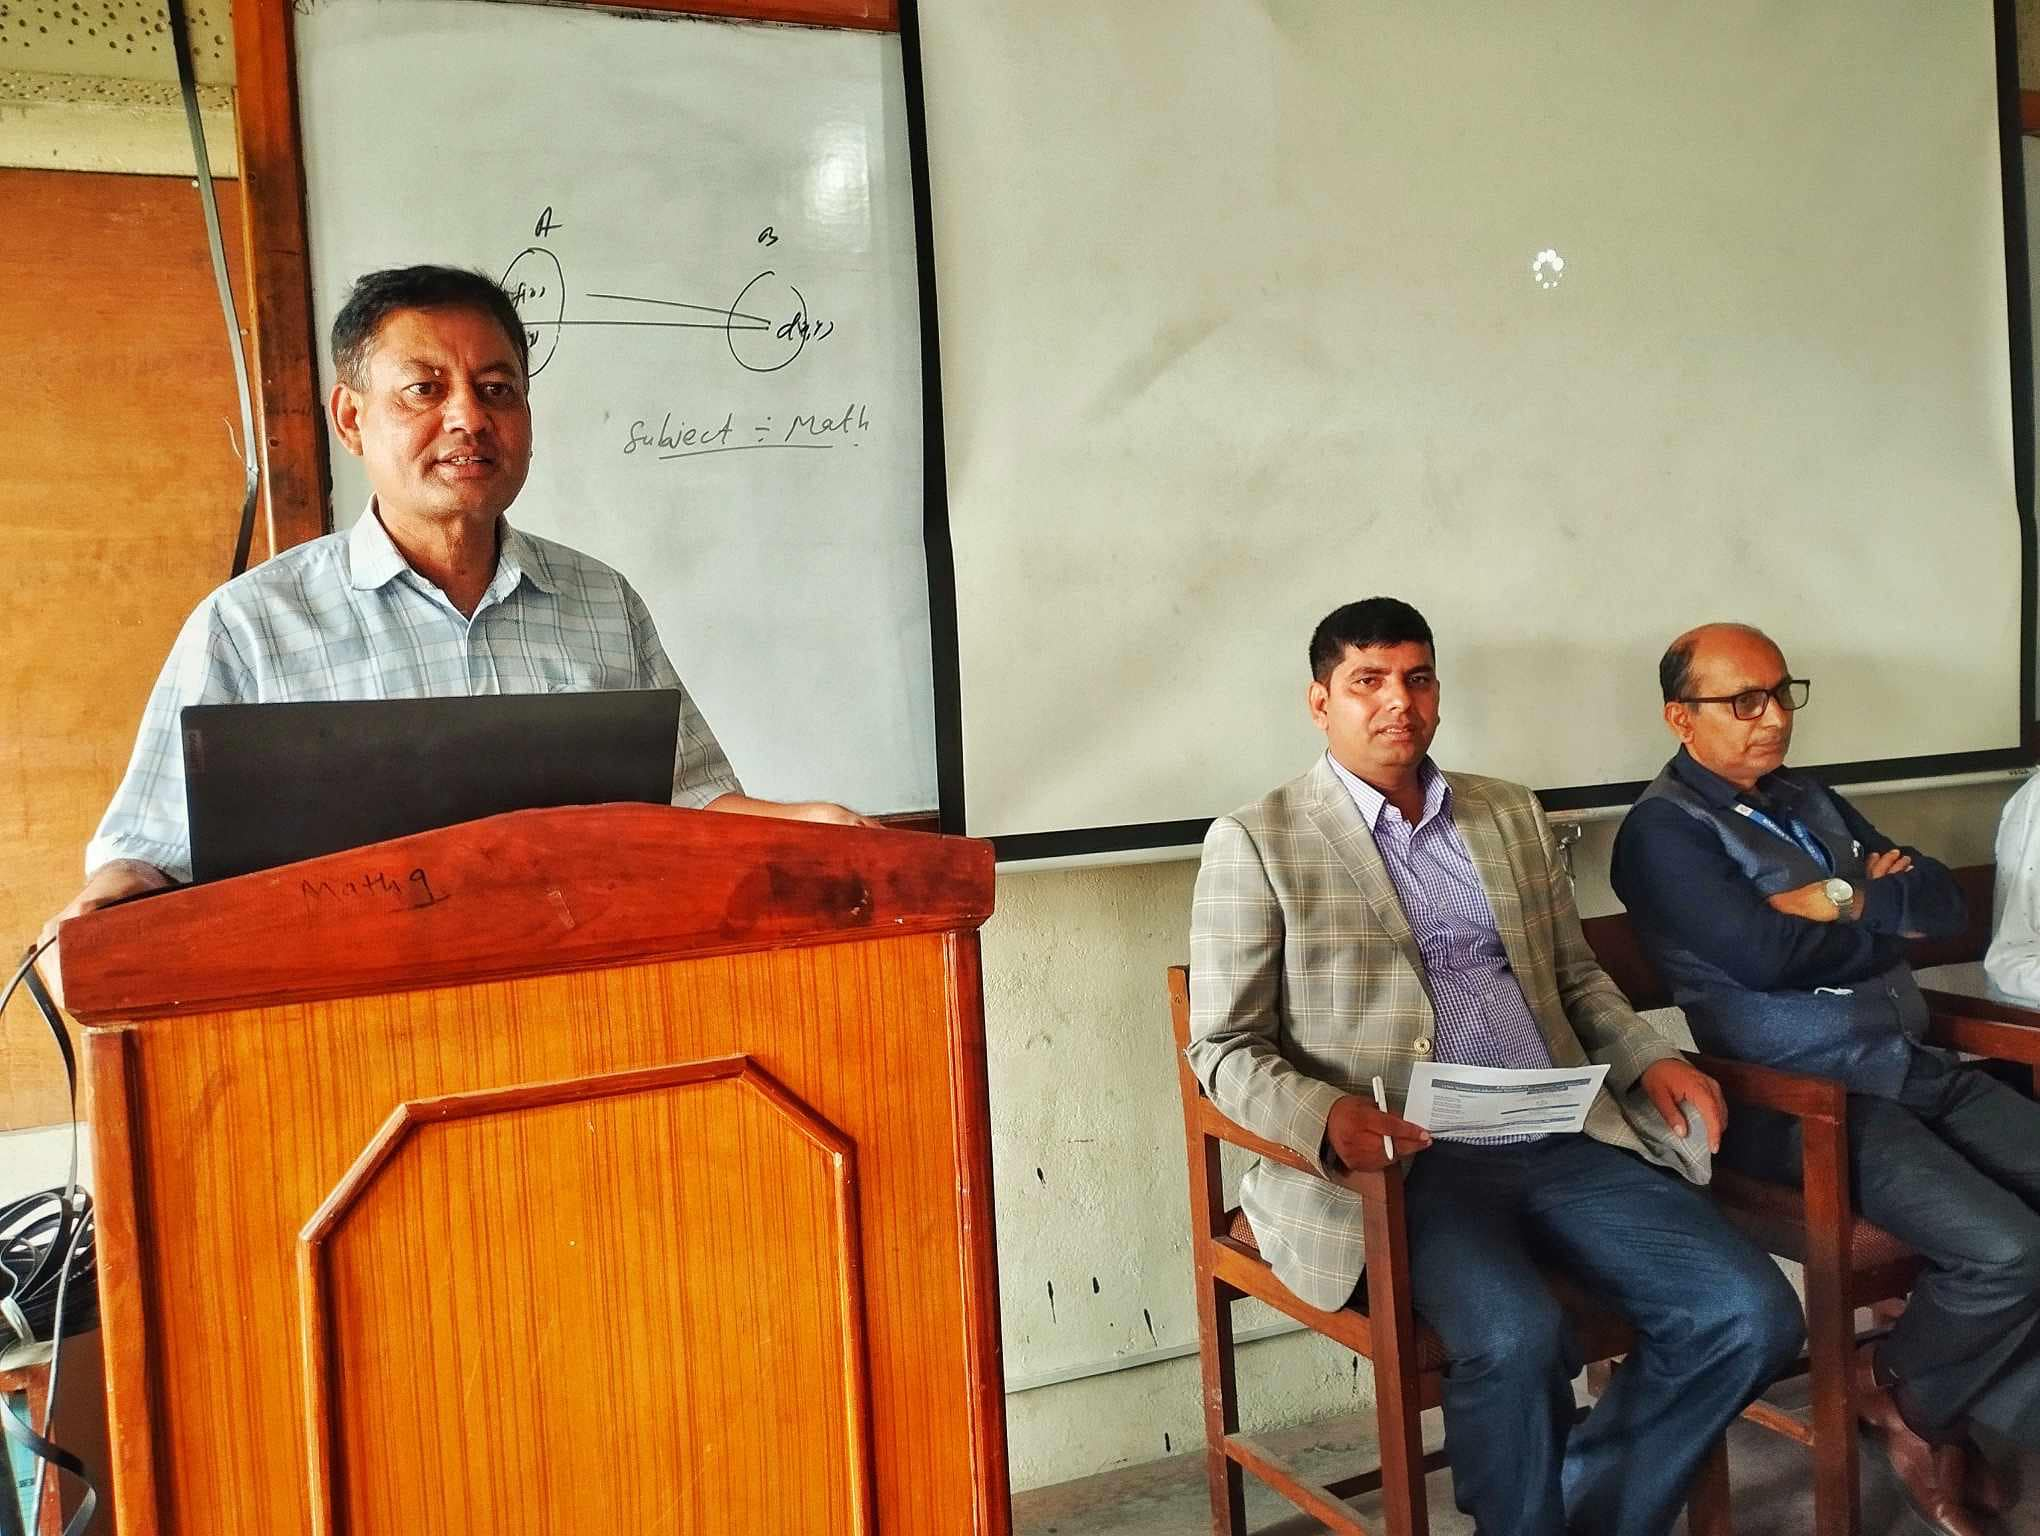
\includegraphics[height=7cm, width=\textwidth]{shreeramsir.jpg}
    \caption{Dr. Khadka}
    \label{fig:first}
\end{subfigure}
\hfill
\begin{subfigure}{0.45\textwidth}
    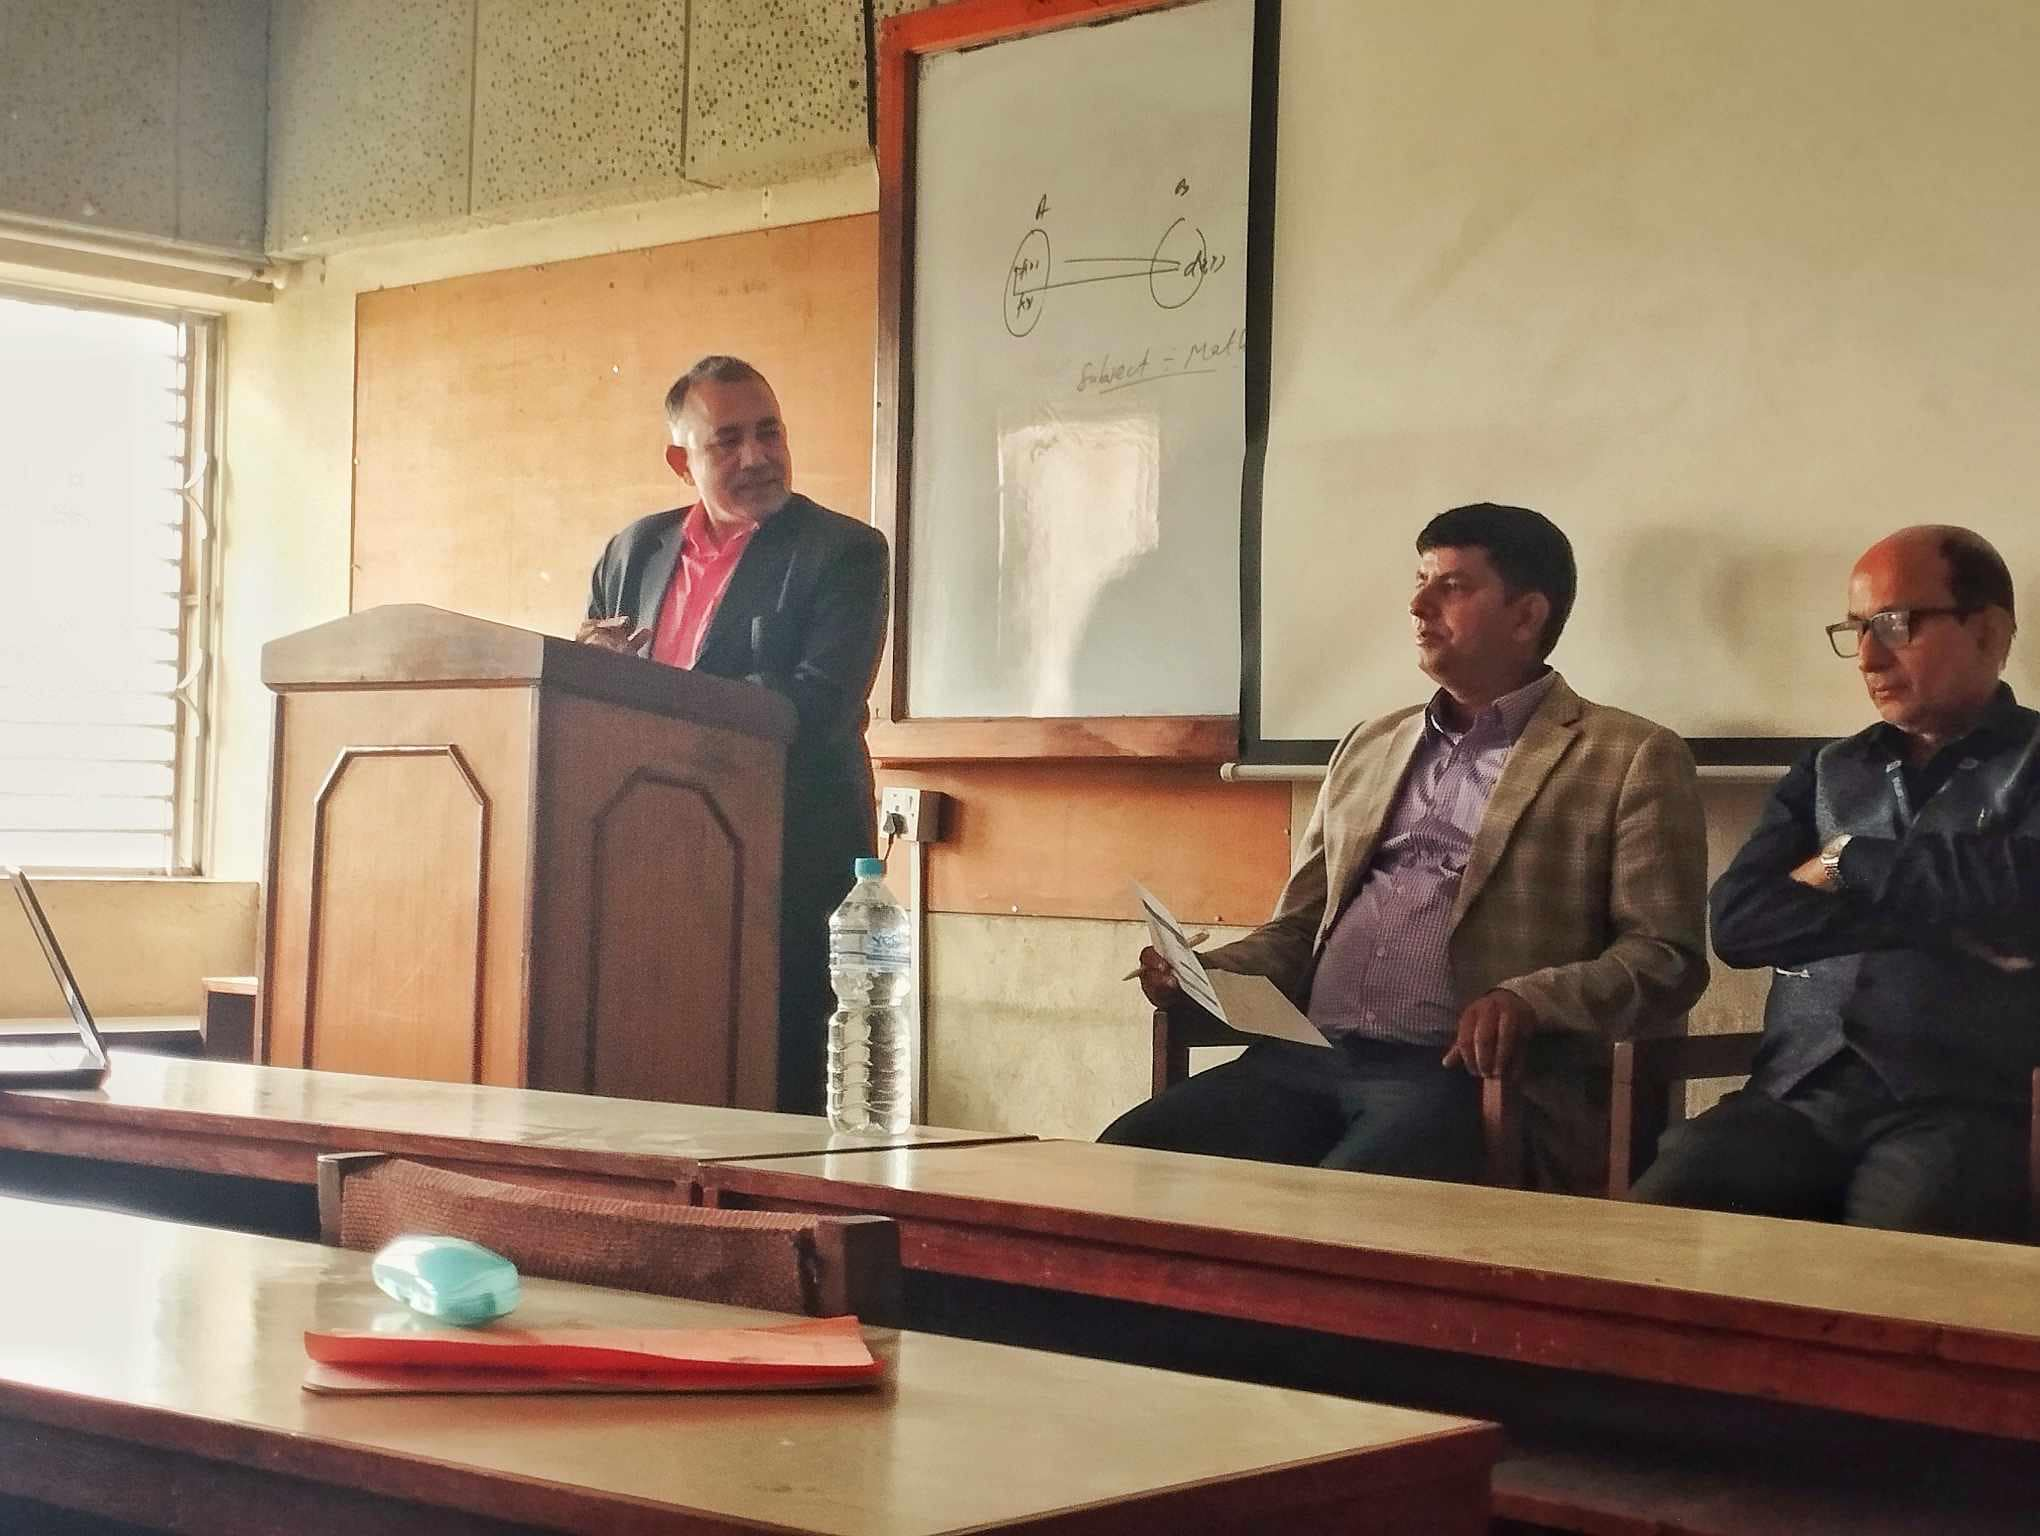
\includegraphics[height=7cm, width=\textwidth]{gyansir.jpg}
    \caption{Dr. Thapa}
    \label{fig:second}
\end{subfigure}
\end{figure}

\noindent
The vice-president of Nepal Mathematical Society Assoc. Prof. Dr. \textbf{Shree Ram Khadka} spoke about the importance of such workshops and gave a big encouragement to the participants and the organizing team.Then he made the participants known about the recently added new grants by the Society to the Mphil and Phd Scholars. The president of the CDM alumni association Prof. Dr. \textbf{Gyan Bahadur Thapa} said such interactions help increase in the member of the association and gave his best wishes to the success of the workshop.\\[3mm]

The newly appointed vice-principal of the Pulchowk Campus, IoST, TU Dr.\textbf{ Puskar Raj Pokharel} said latex can be difficult learn in the beginning and talked about the challenges of learning latex in old times when there was no good internet and technology. He also talked about the advantages of using latex which is a powerful markup languages over word-processors as MS-word. Latex has significant advantages in typesetting math symbols over the word-processors.

\begin{figure}[h!]
  \centering
  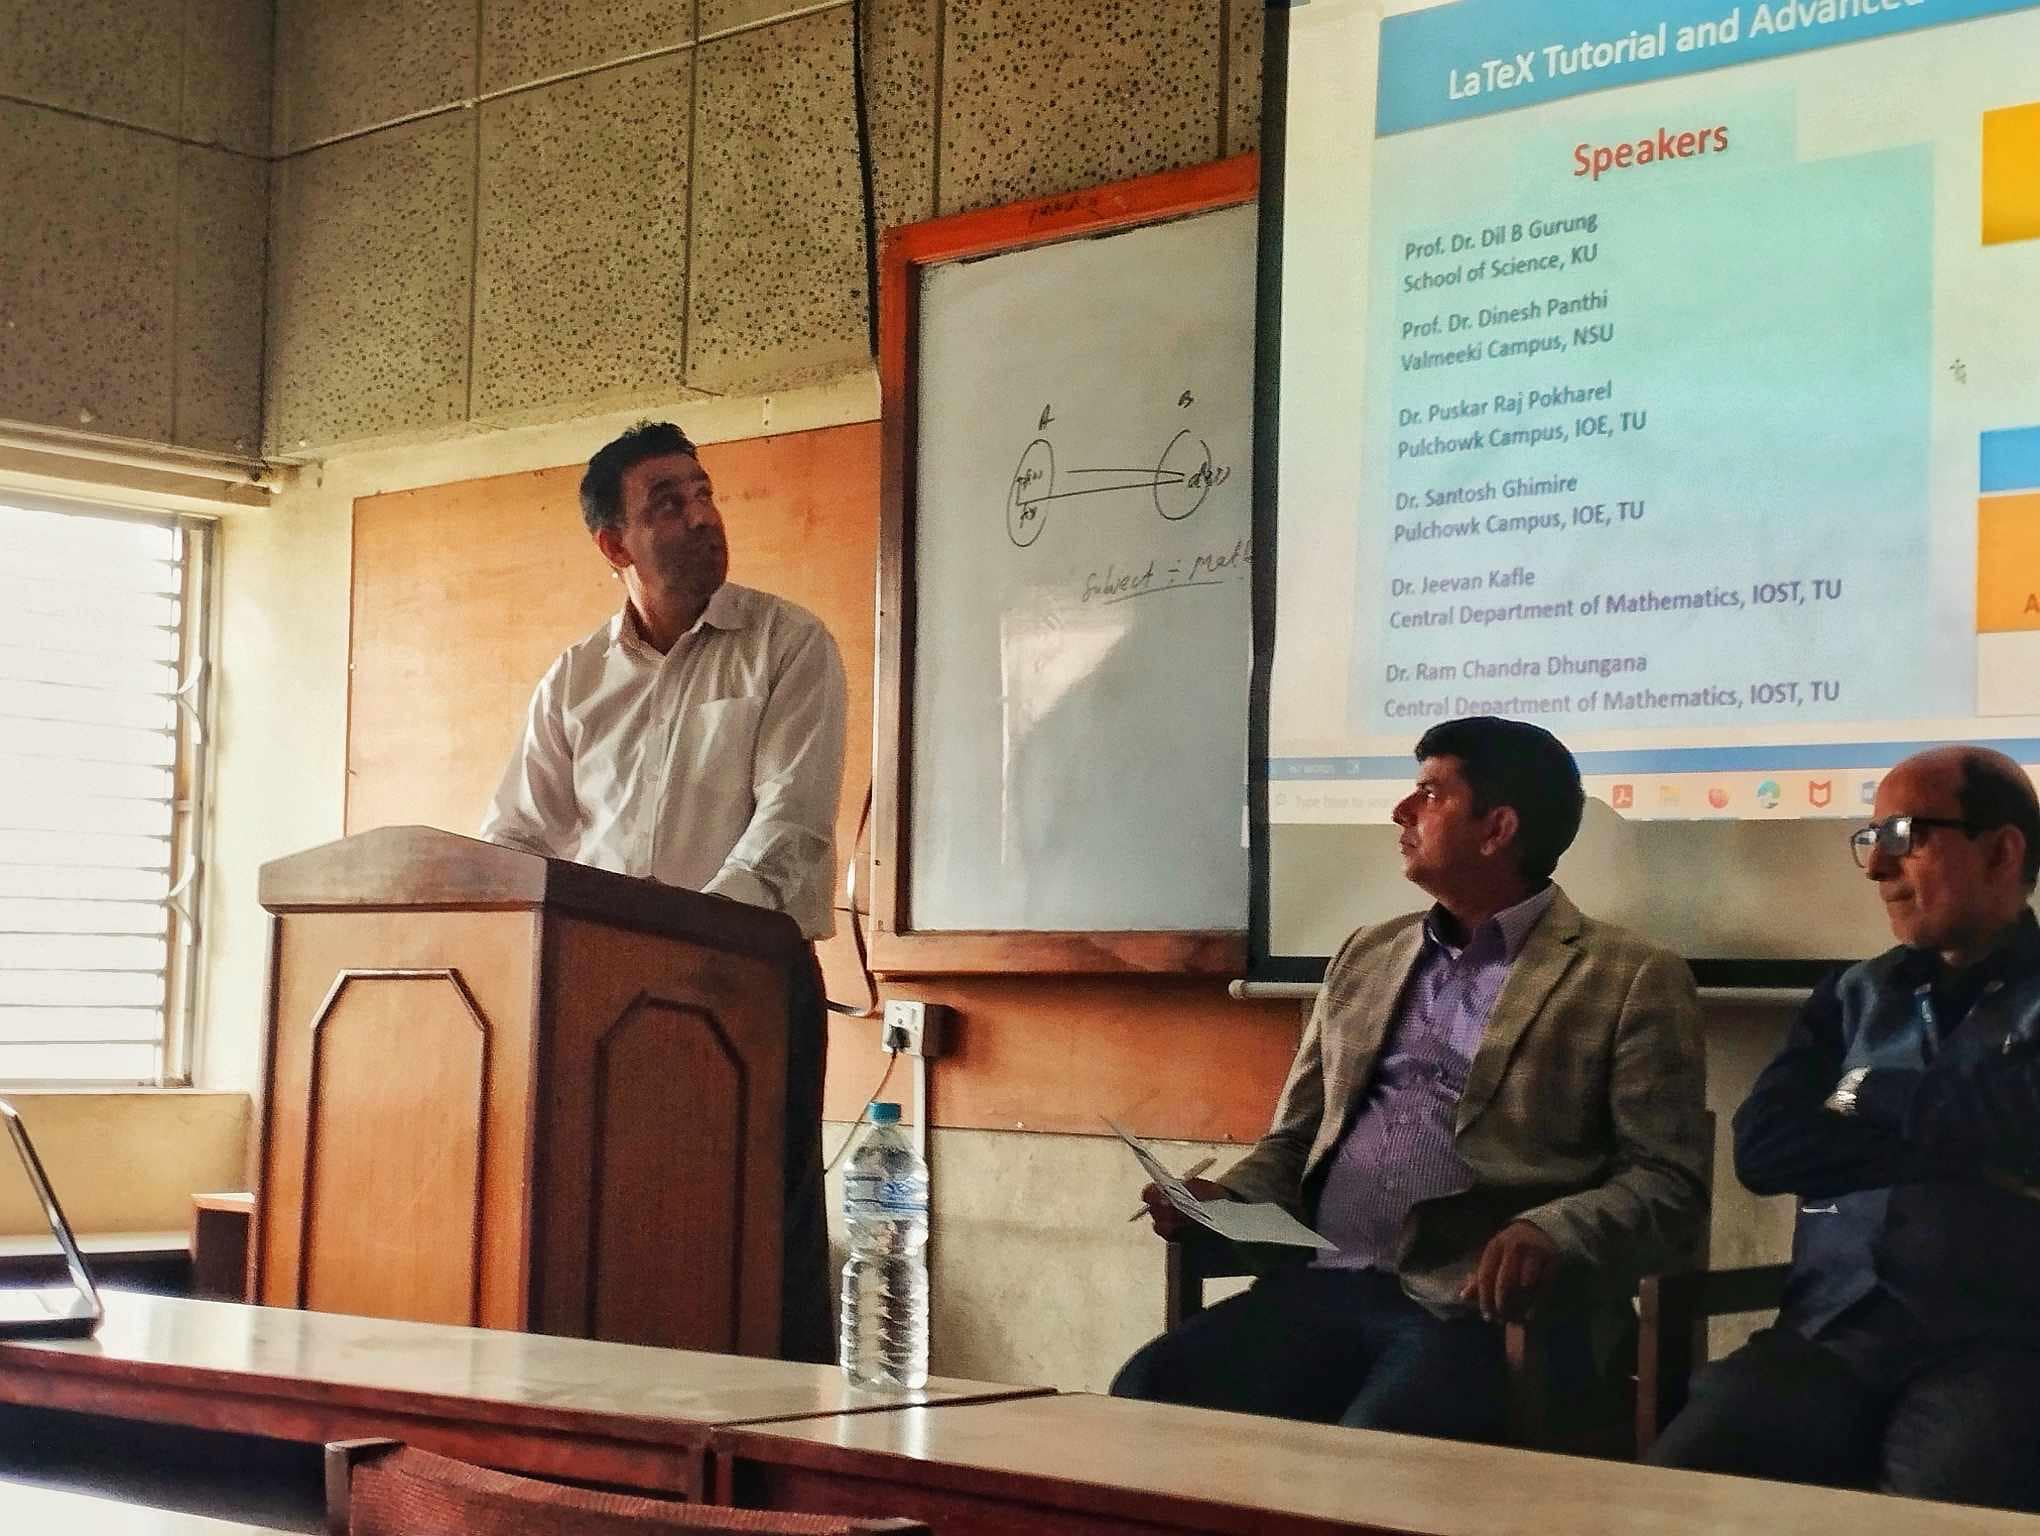
\includegraphics[height=6cm, width=9cm]{puskarsir2.jpg}
  \caption{Dr. Puskar Raj Pokharel}
\end{figure}
\clearpage

\begin{center}
  {\bfseries \Large Day 1, 20-Baishakh, Thursday}
\end{center}
\vspace{3mm}

{\bfseries \large Sessioin 1}\\[3mm]
The first expert of this session was Dr. \textbf{Ram Chandra Dhungana} and Dr. \textbf{Kafle}. Dr. Dhungana trained the participants on the \textit{Basics of Latex, Creation of a Latex document and Mathematics in Latex}.
\vspace{3mm}

\begin{figure}[h!]
  \centering
  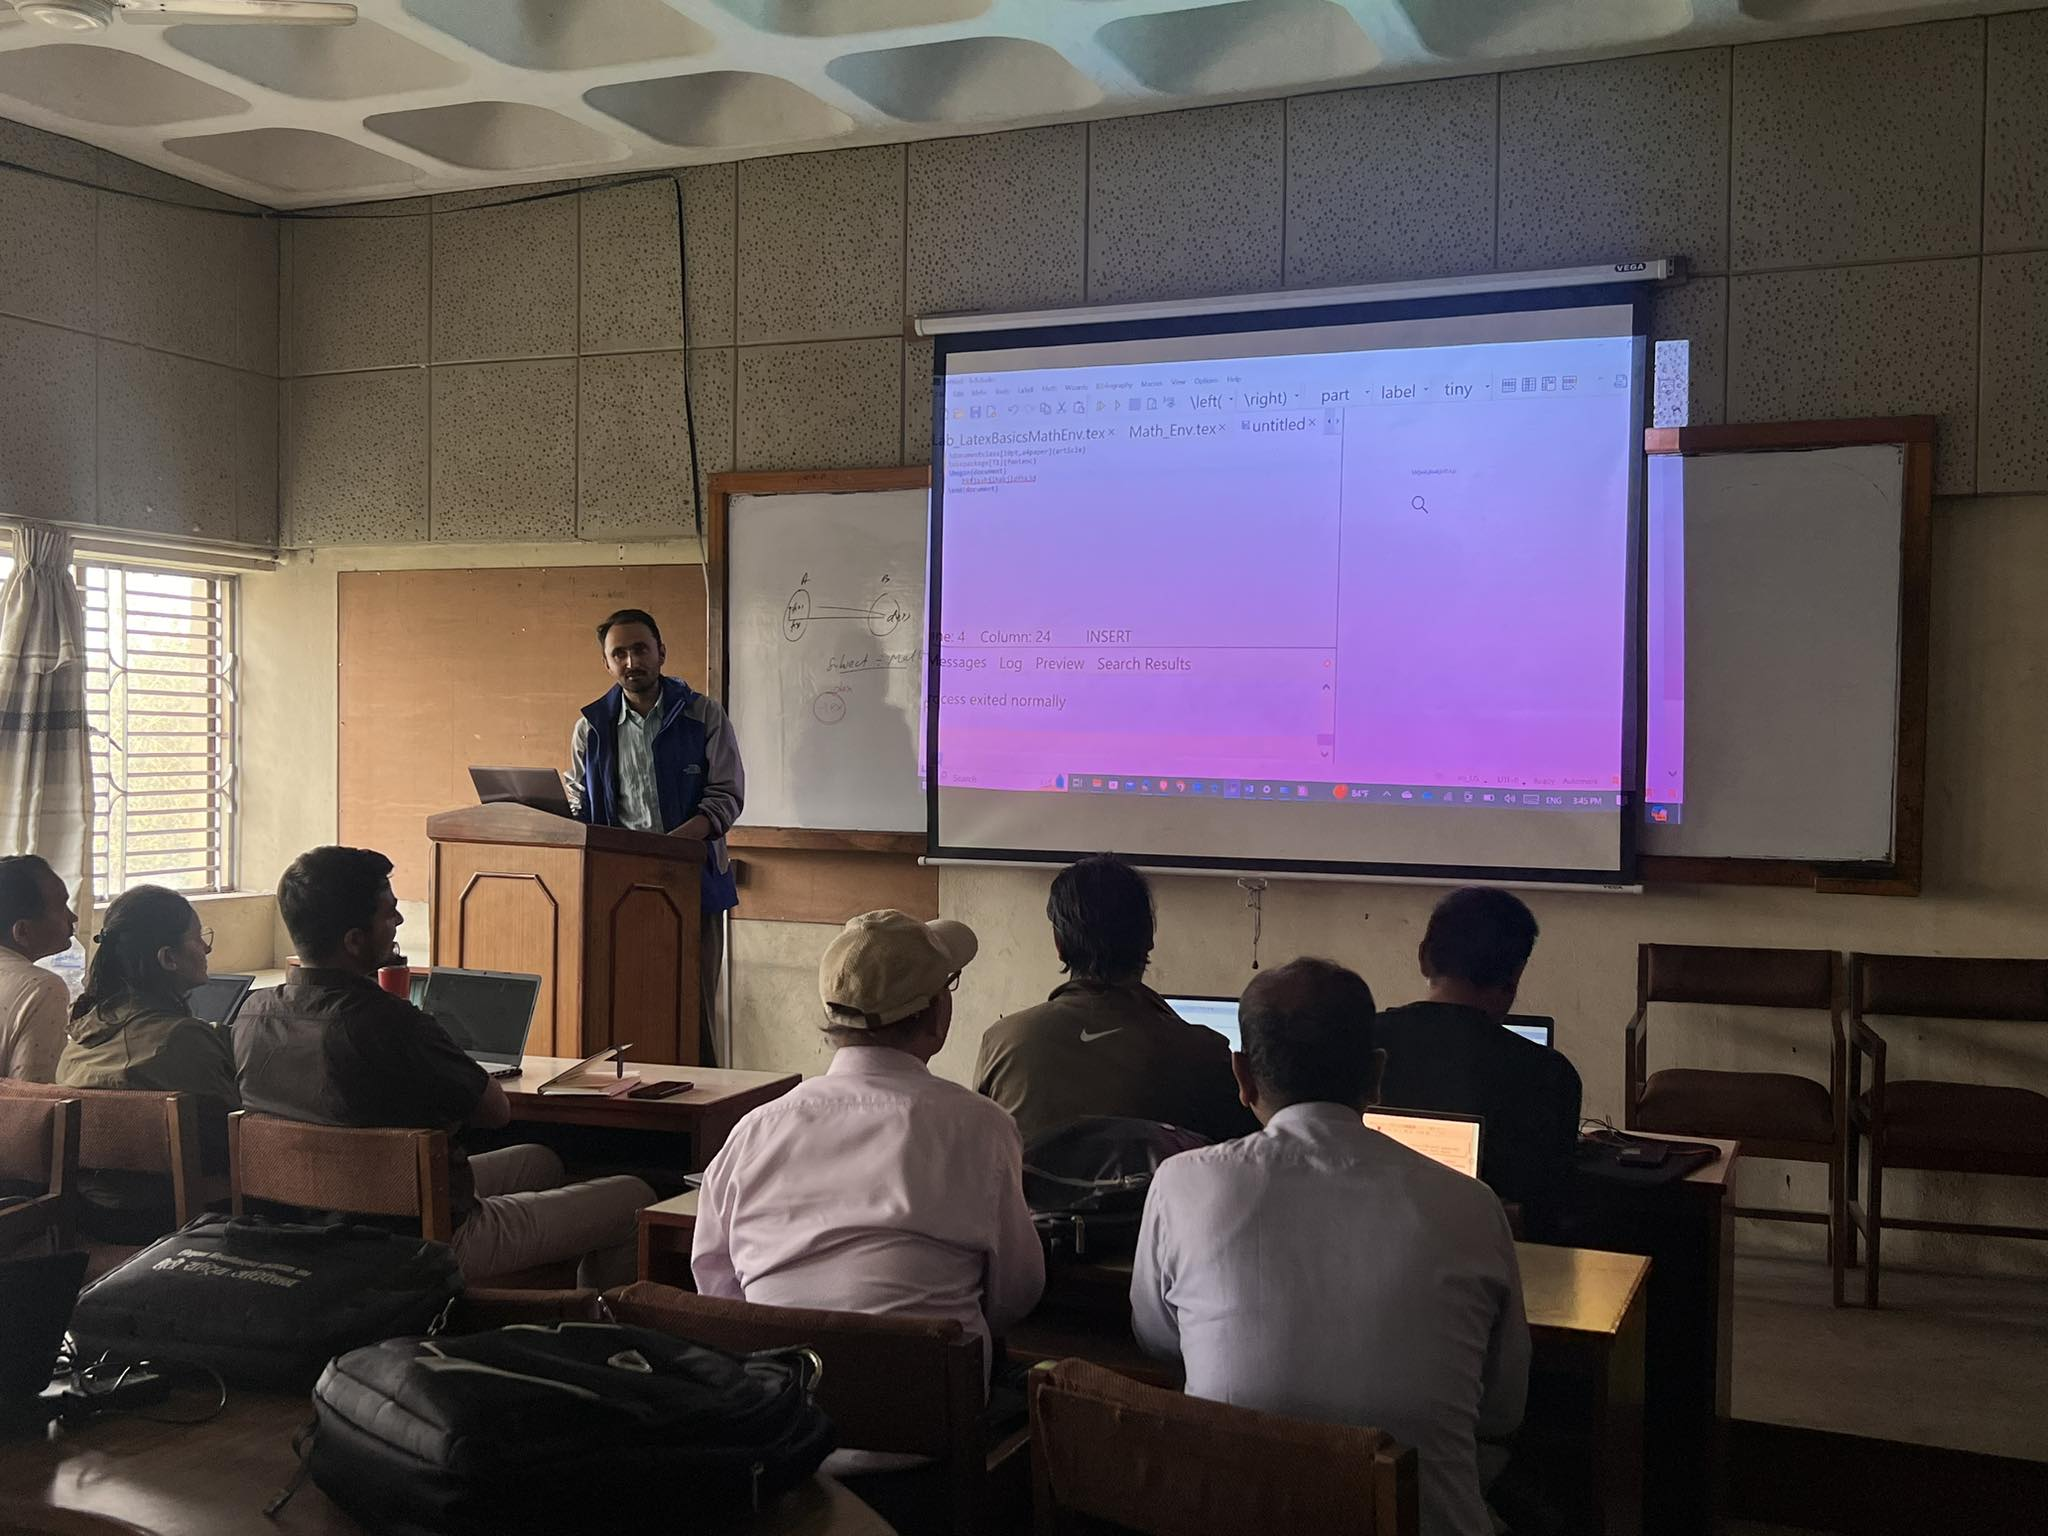
\includegraphics[height=7cm, width=9cm]{rcd.jpg}
  \caption{Dr. Ram Chandra Dhungana}
\end{figure}
\vspace{2mm}
The workshop broke for snacks at 5:30pm.

\vspace{5mm}

{\bfseries \large Session 2}\\[3mm]
The expert of this session was the vice-principal of Pulchowok Campus, Dr. \textbf{Puskar Raj Pokharel}. He trained the participants on the two important aspects of the latex document \textit{Including Graphs and Placing Figures and Preparing Bibliography}.
\vspace{3mm}

\begin{figure}[h!]
  \centering
  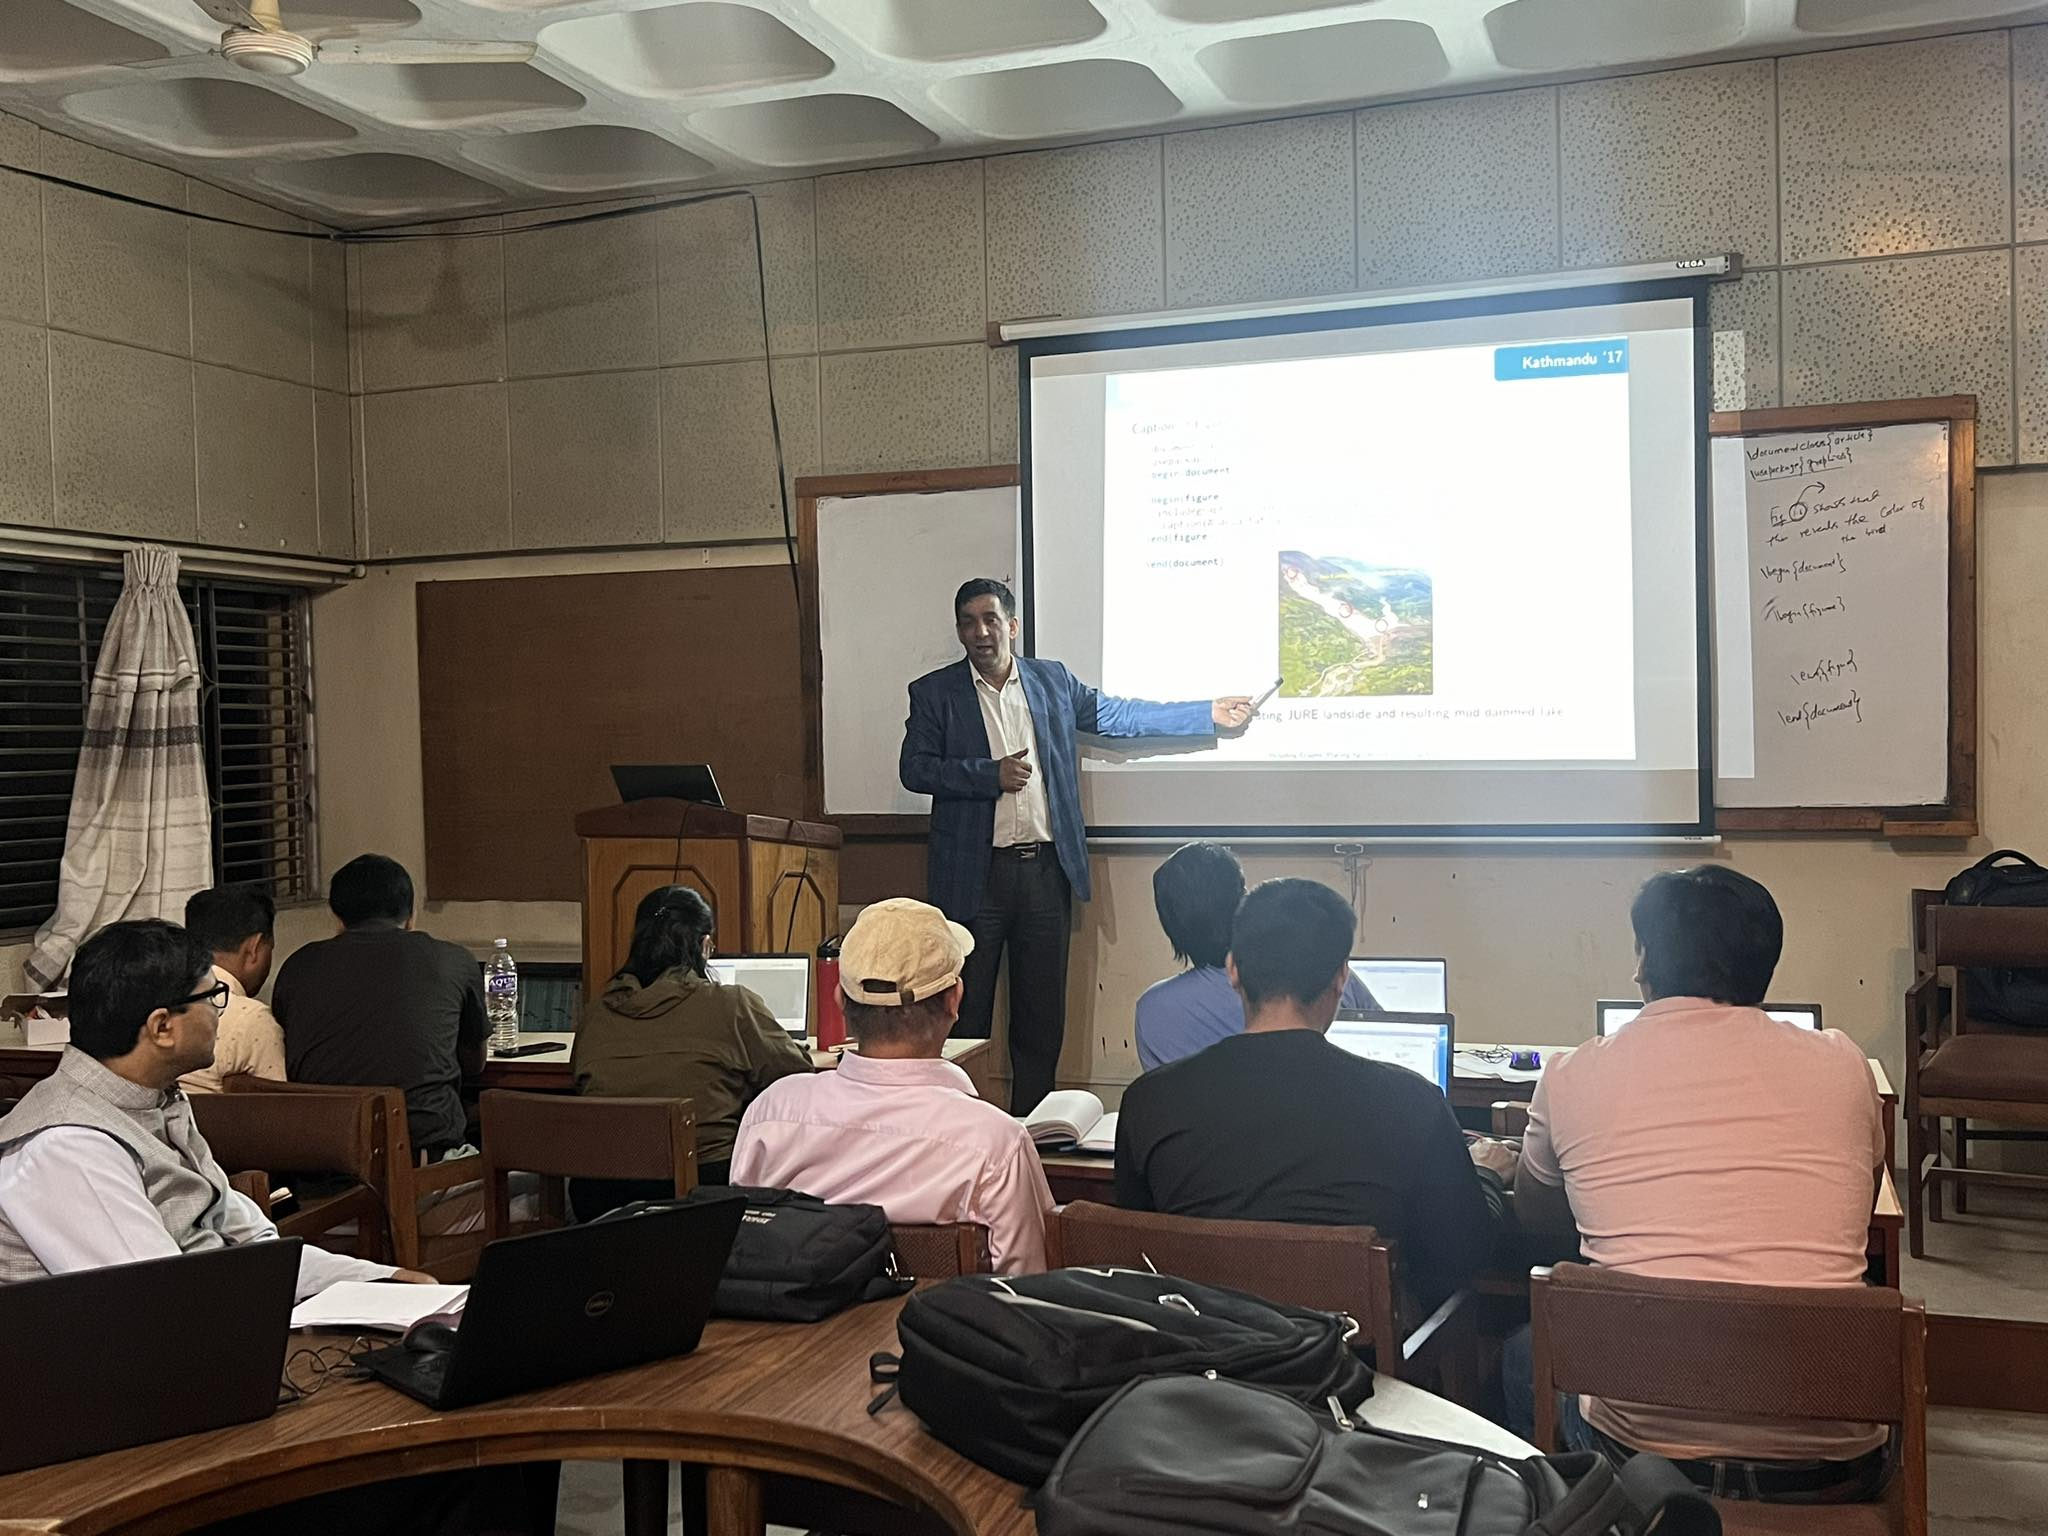
\includegraphics[height=7cm, width=9cm]{puskar.jpg}
  \caption{Dr. Puskar Raj Pokharel}
\end{figure}
\clearpage

\begin{center}
  {\bfseries \Large Day 2, 21-Baishakh, Friday}
\end{center}
\vspace{3mm}

{\bfseries \large Session 3 : Online session}\\[3mm]
The session was from 7pm to 9pm online. The special guest of this session was the principal of RR Campus, Dr. \textit{Jivan Jnawali}.  This session was done via zoom-meeting so it was open to all. The expert of this session was Dr. \textbf{Dil Bahadur Gurung} of School of Science, KU. He trained the participants \textit{About the Template of the Nepali Mathematical Sciences Report /JNMS}. JNMS stands for the Journal of Nepal Mathematical Society.

\begin{figure}[h!]
\centering
\begin{subfigure}{0.45\textwidth}
    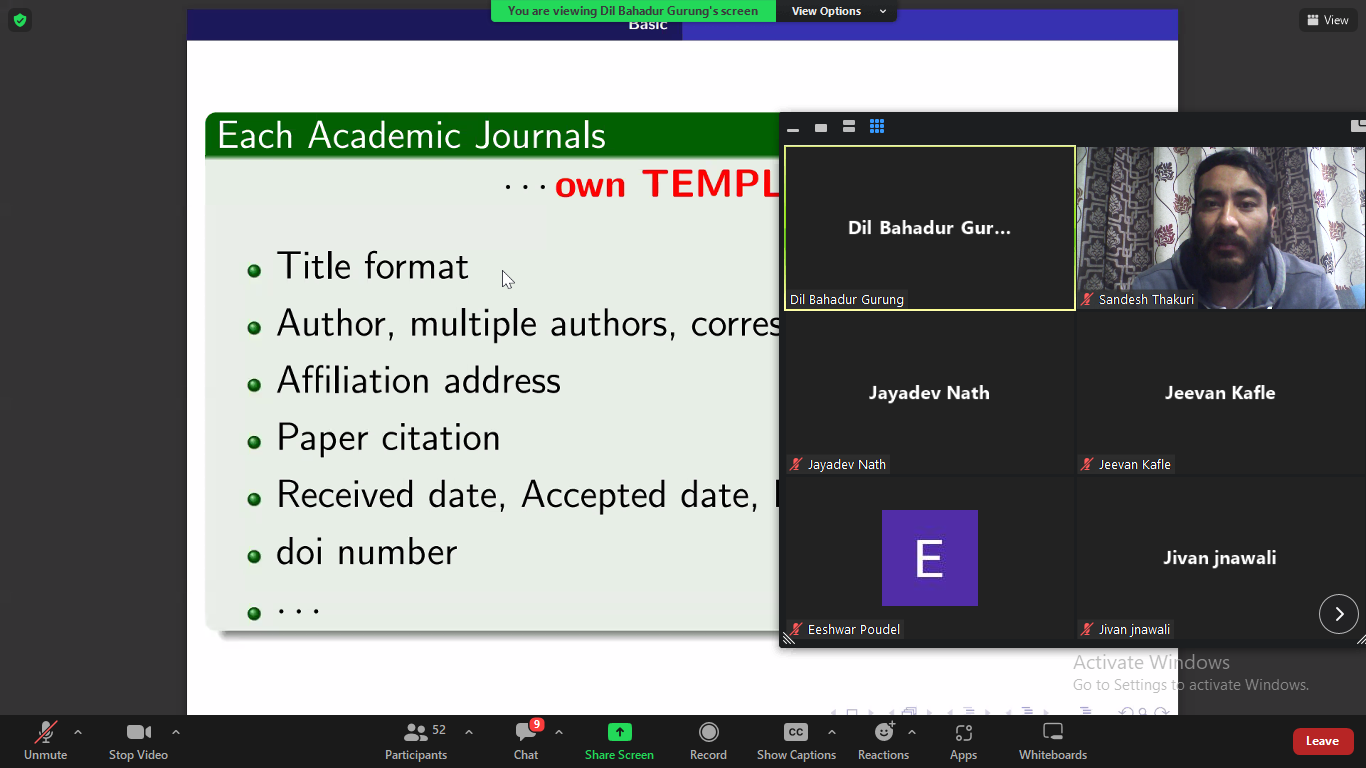
\includegraphics[height=5cm, width=\textwidth]{online1.png}
\end{subfigure}
\hfill
\begin{subfigure}{0.45\textwidth}
    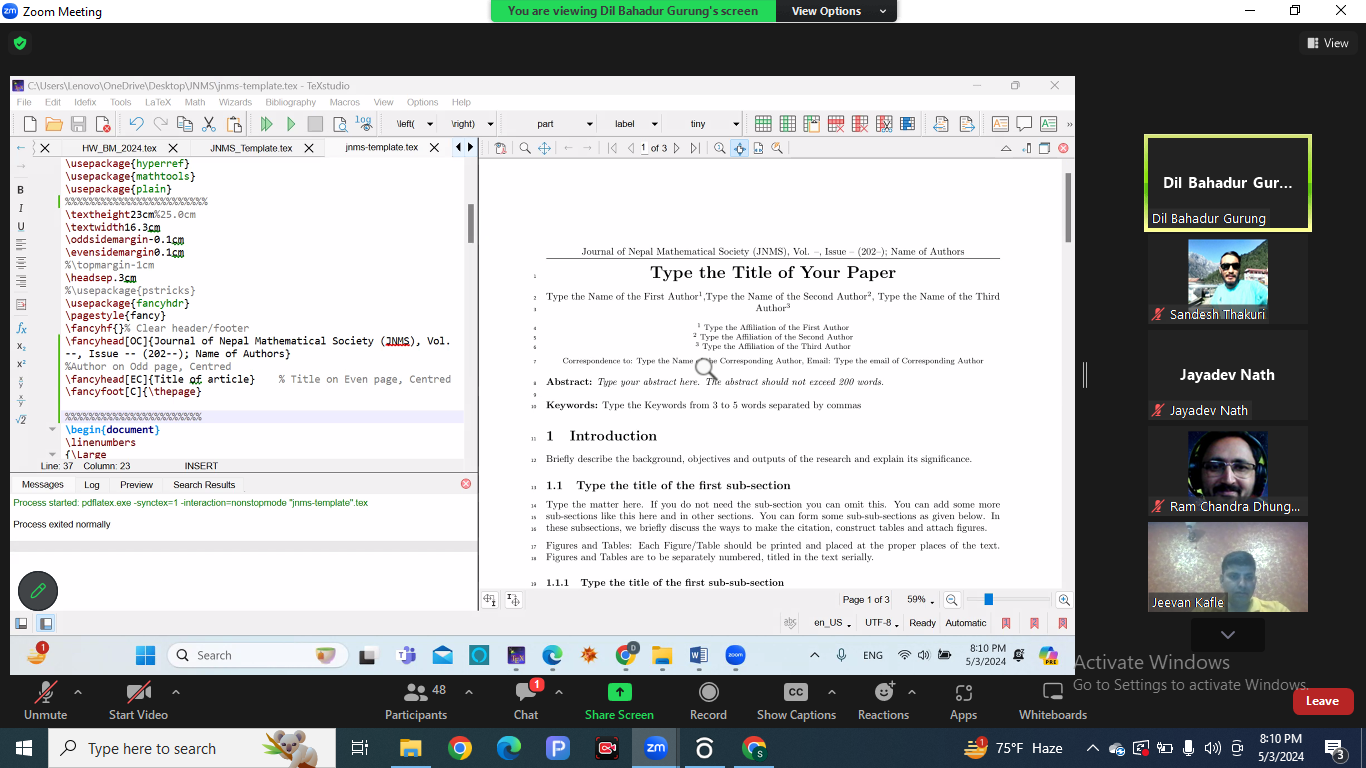
\includegraphics[height=5cm, width=\textwidth]{online2.png}
\end{subfigure}
\end{figure}

The templates of most scientific journals are done in latex including the JNMS. This is why latex is crucial. He mentioned that even a good research article may be rejected if not submitted in latex. He shared a story of his friend whose good research article was rejected simply because it was not done in latex. He showed the participants the template of JNMS and instructed the participants the following.
Each journal has its own template. The template has its parts: Title, Author, Affiliation, Abstract, Main Body, Conclusion, Citation format etc. To format a article for a specific journal first visit its website and read the instructions for authors and download a latest article published to get the feel. Then download the template and work on it. Reference format and citation format are challenging aspects of article writing.
The session was ended with the questions from the participants and feedback from the special guest Dr. Jnawali.

\begin{figure}[h!]
  \centering
  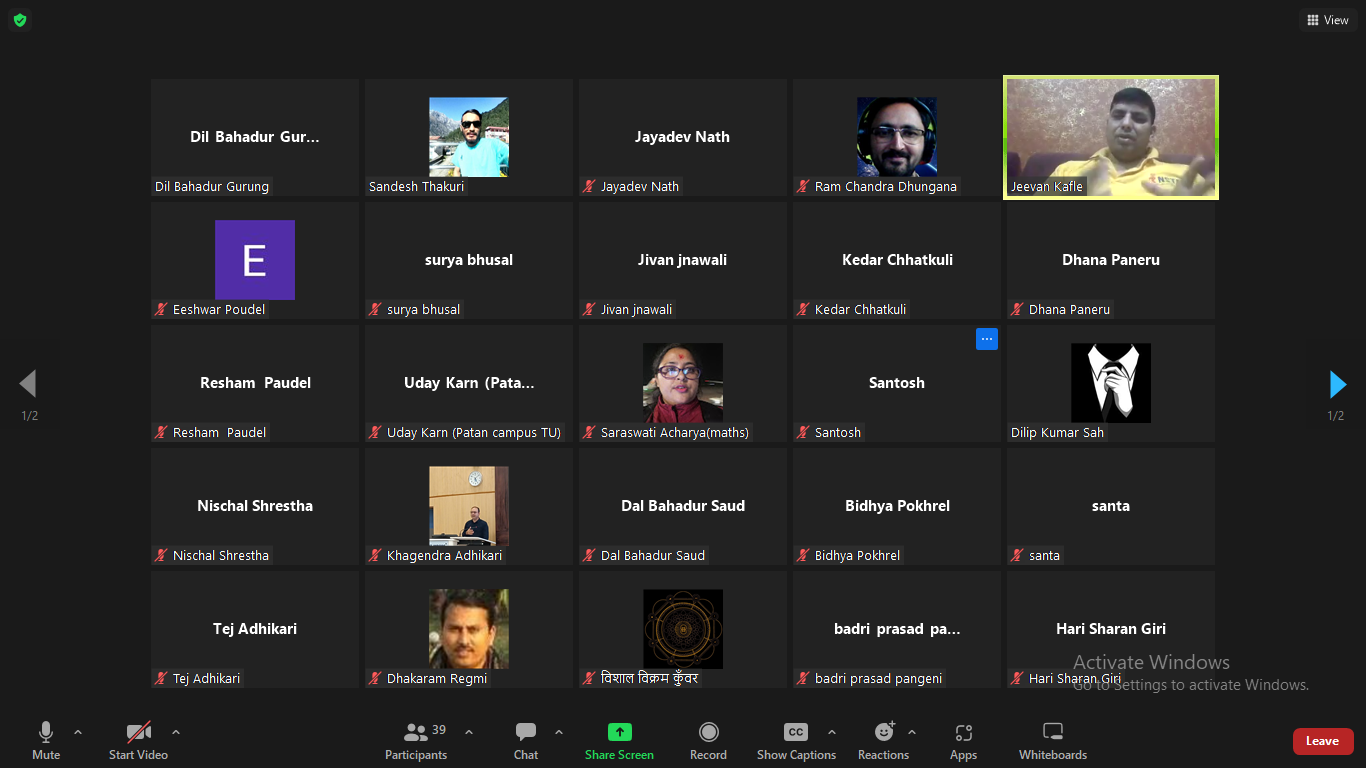
\includegraphics[height=7cm, width=15cm]{online3.png}
\end{figure}
\clearpage


\begin{center}
  {\bfseries \Large Day 3, 21-Baishakh, Saturday}
\end{center}
\vspace{3mm}

Before the fourth session Dr. Pokharel gave a quick revision to the participants from 11am to 12pm.\\

{\bfseries \large Session 4}\\[3mm]
The expert of this session was Dr. \textbf{Santosh Ghimire} of Pulchowk Campus, TU and Dr. \textbf{Kafle}. Dr. Ghimire trained the participants on \textit{Tabular Material and Document Layout}. First he taught the participants how to set the margins in a latex document which is generally done using the ``geometry package'' of the latex. This was followed by the document organization: chapter, section, subsection, paragraph, list, etc. Then he moved on to creating and placing of a tabular material in a latex document. Participants were given sufficient time to practice on their own. At ended he showed some tricks in latex. Mr. \textbf{Sandesh Thakuri} continued the session giving a talk on drawing graphics in latex using the package \textit{tikzpicture}. He made a flowchart using tikzpicture.
\vspace{7mm}

\begin{figure}[h!]
\centering
\begin{subfigure}{0.48\textwidth}
    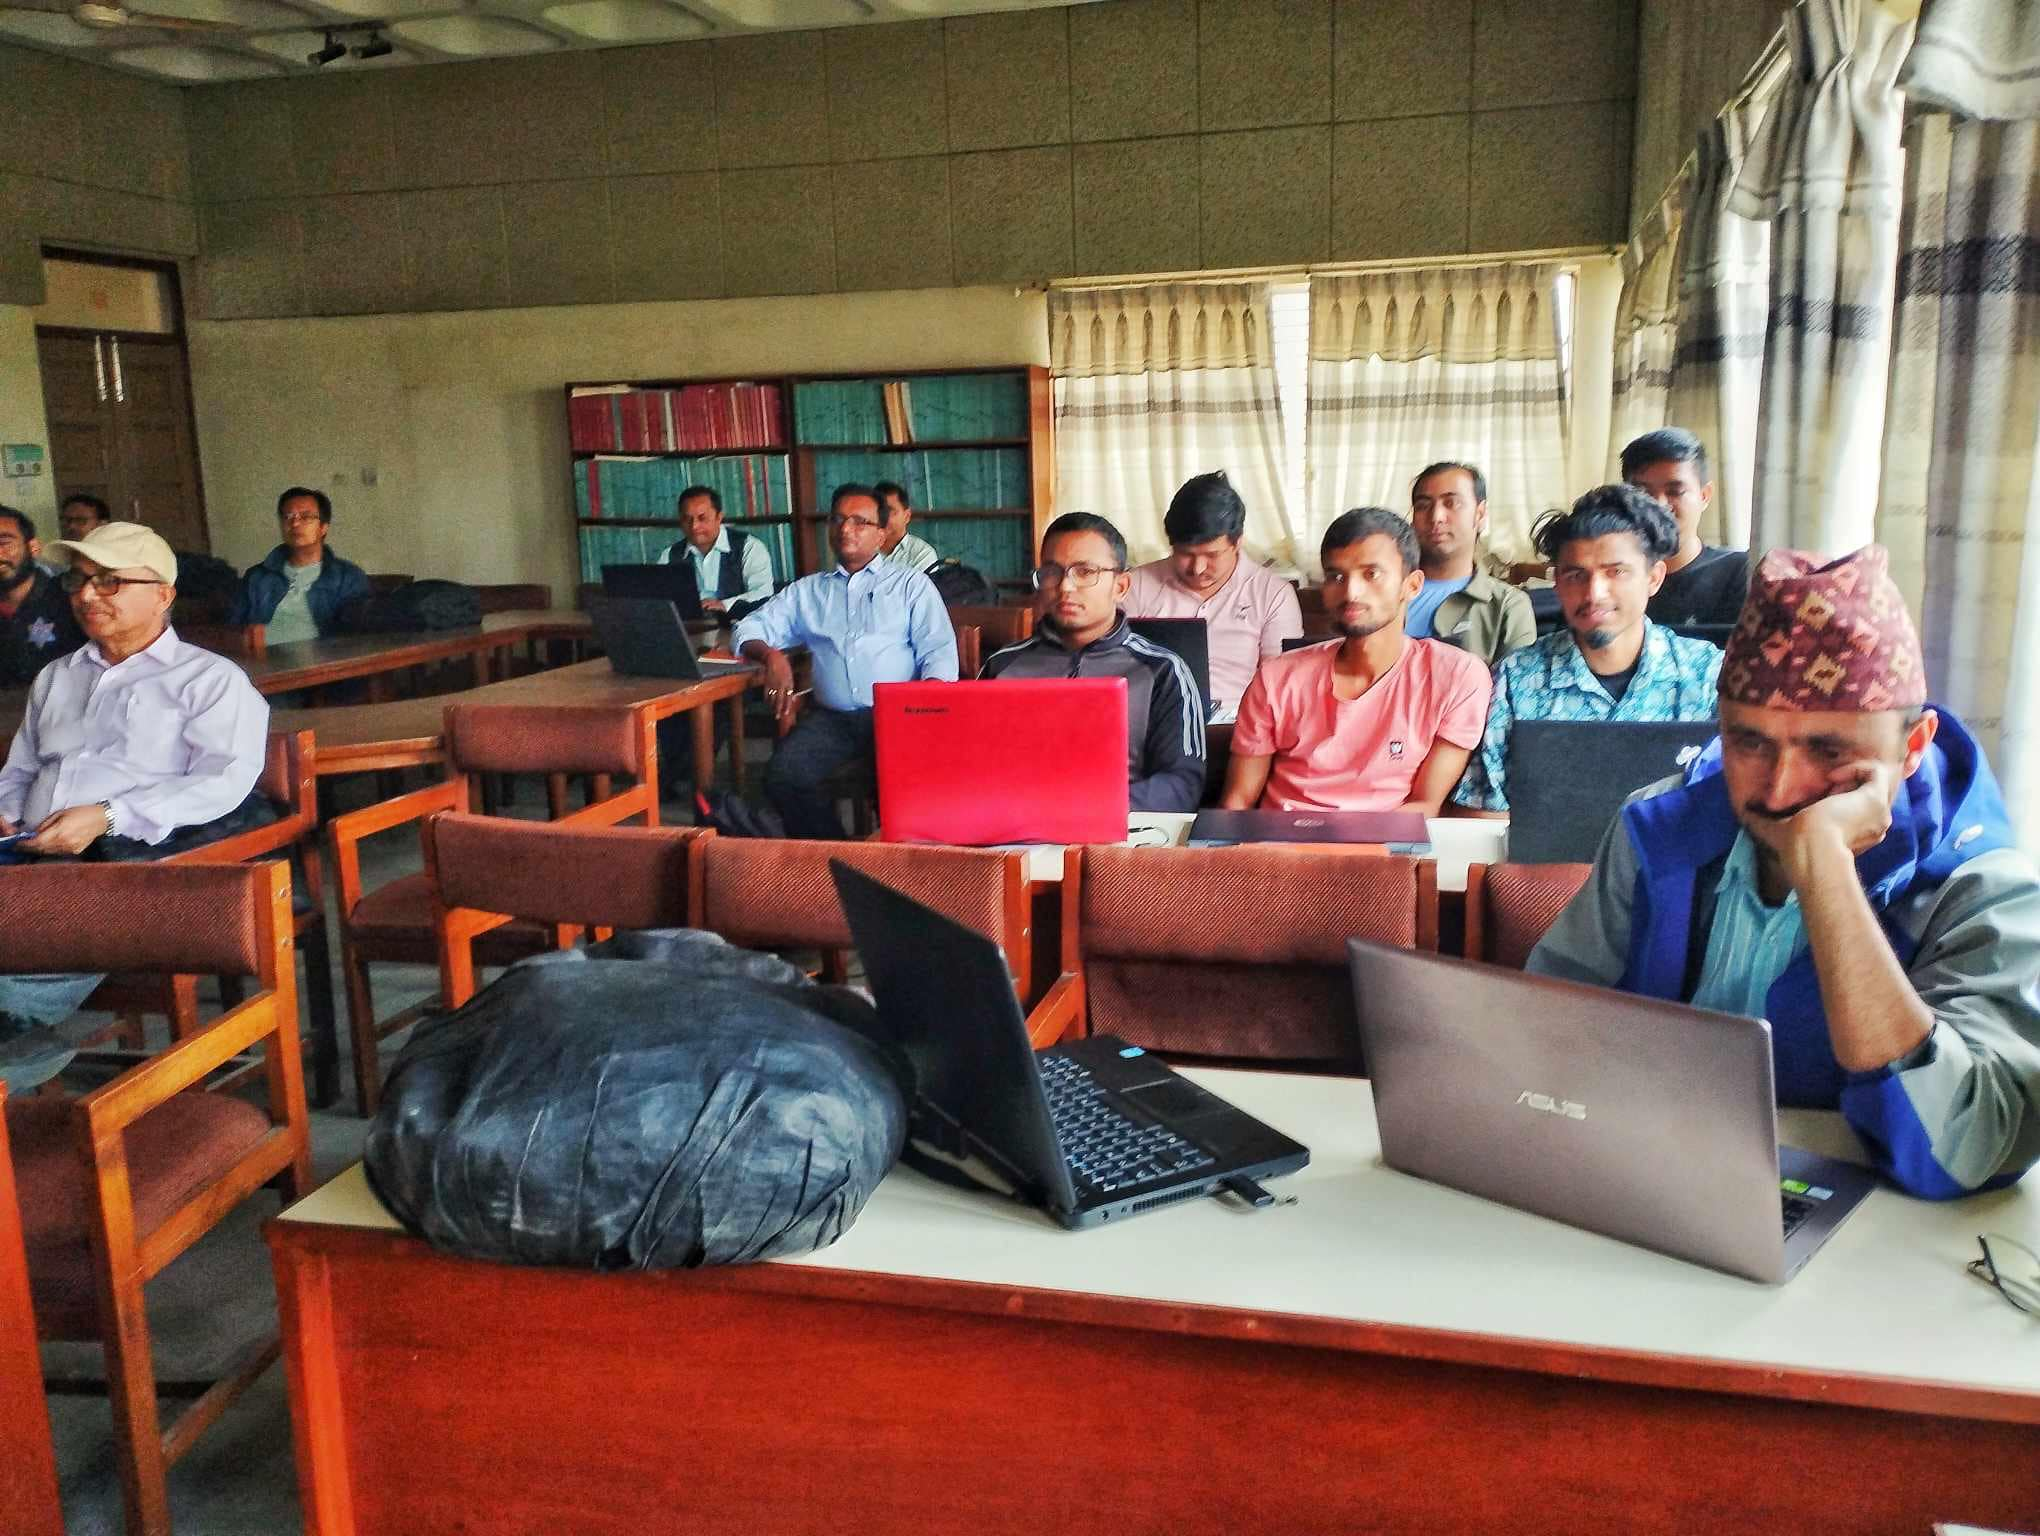
\includegraphics[height=6cm, width=\textwidth]{santosh.jpg}
\end{subfigure}
\hfill
\begin{subfigure}{0.48\textwidth}
    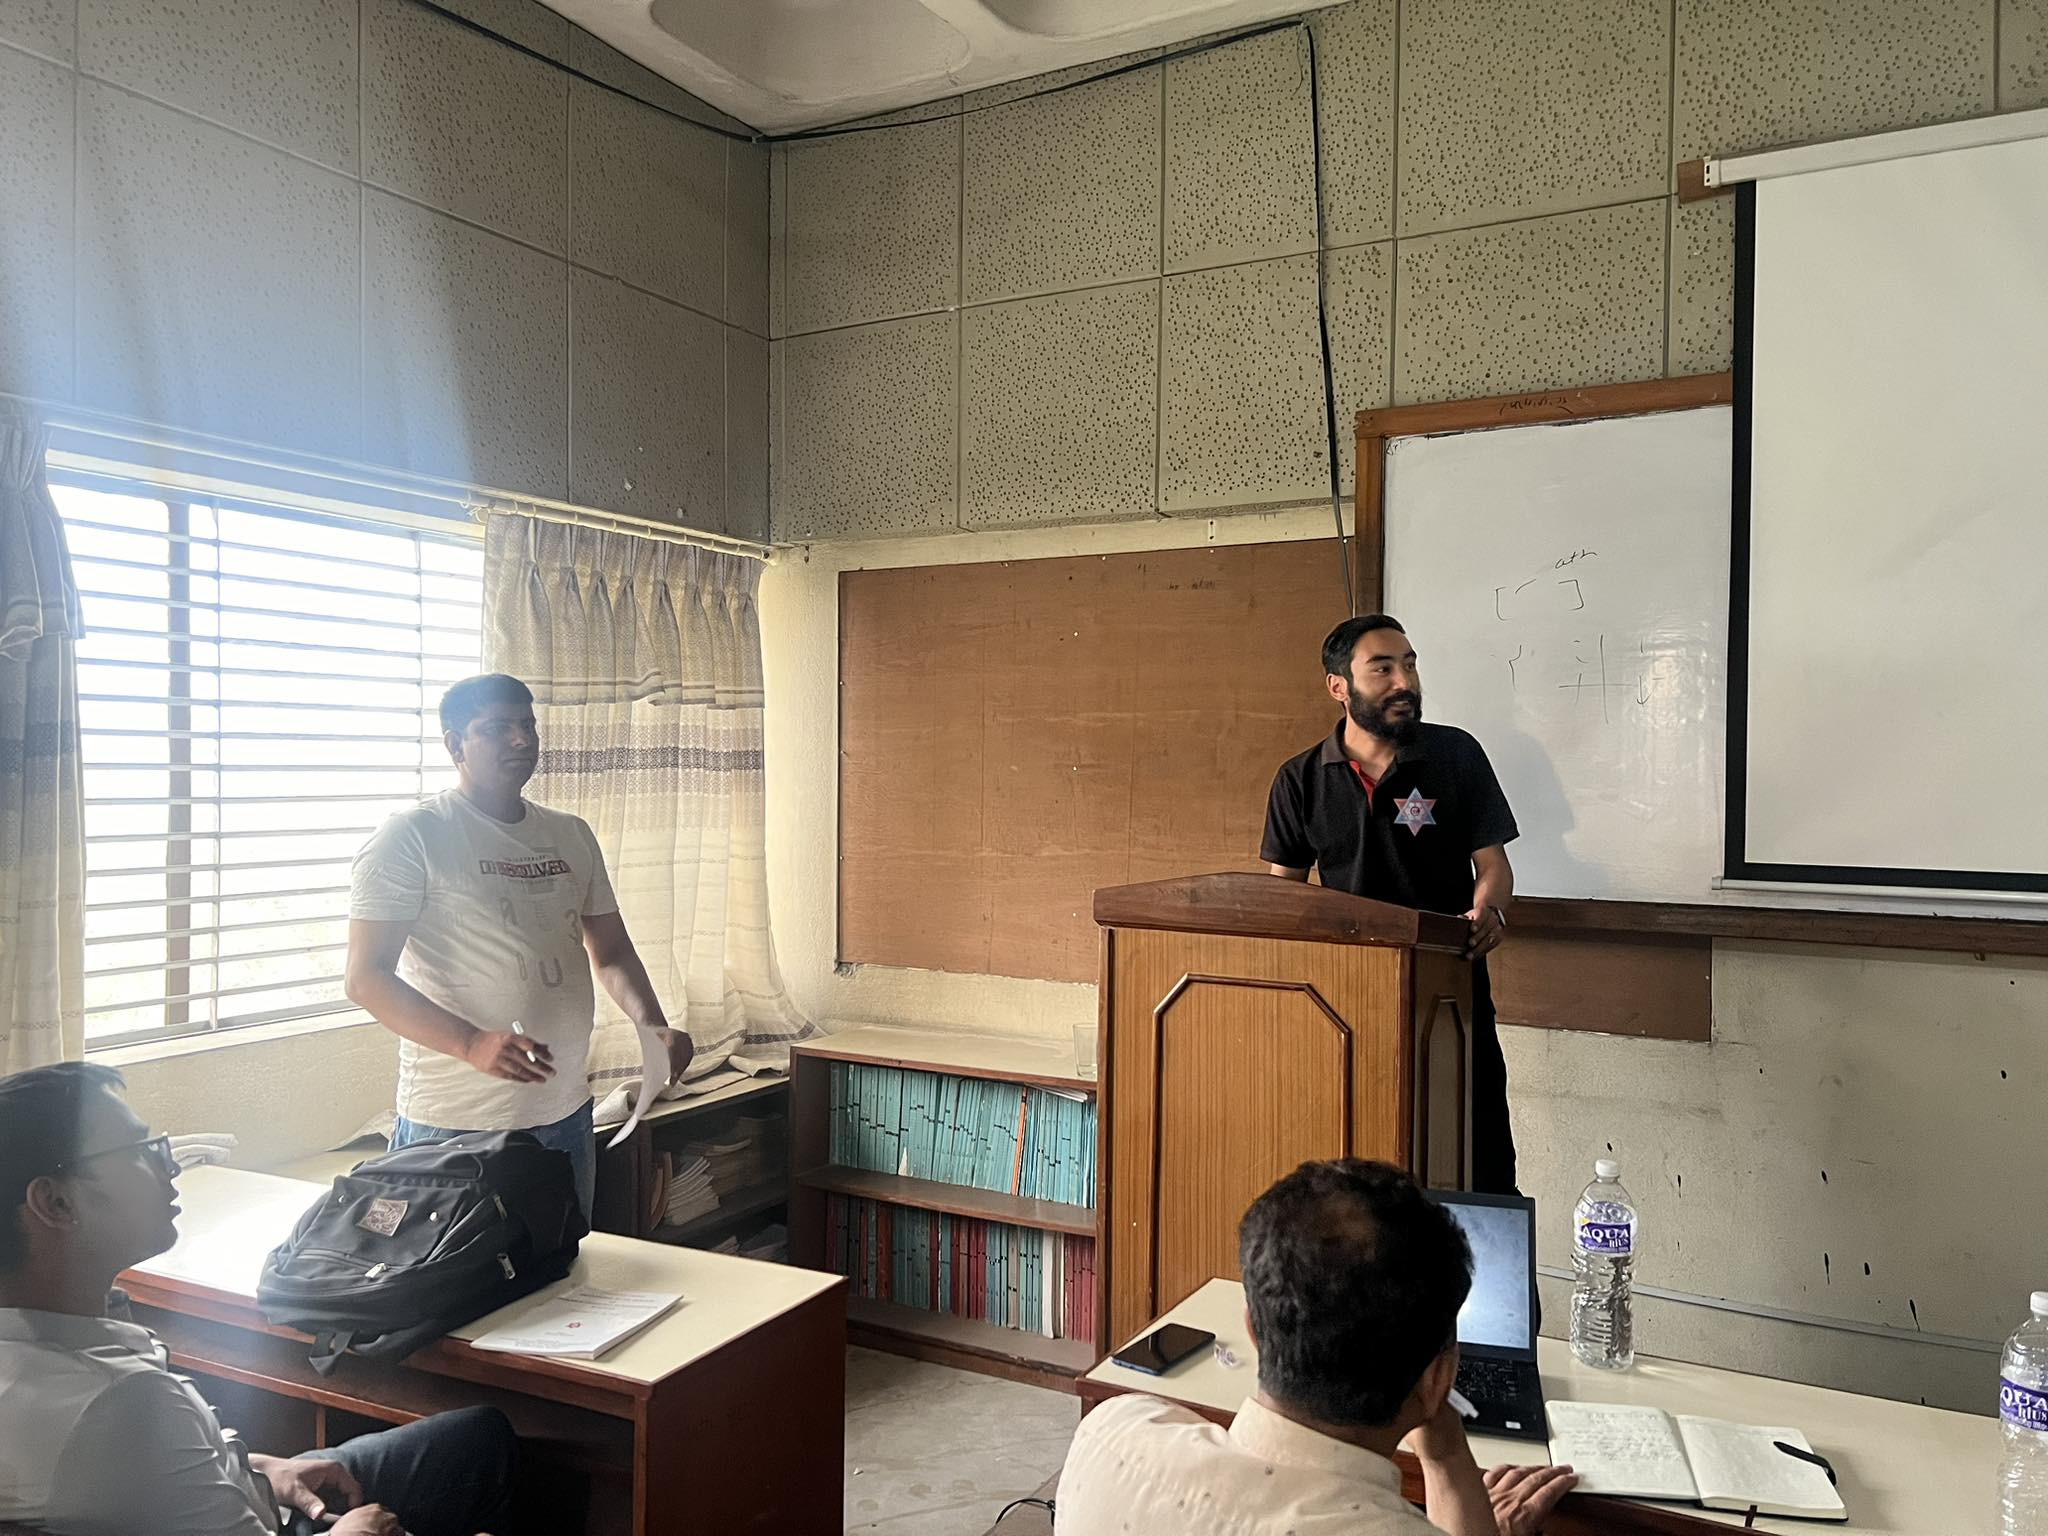
\includegraphics[height=6cm, width=\textwidth]{sandesh2.jpg}
\end{subfigure}
\end{figure}

\vspace{7mm}
{\bfseries \large Session 5}\\[3mm]
The expert of this session was Dr. \textbf{Dinesh Panthi} of Valmeeki Campus, Nepal Sanskrit University. Dr. Panthi trained the participants on \textit{Presentation in Beamer}. Beamer is a document class in latex. It allows us to create slides and frames which is a presentation tool in latex. This is a popular class used by the researchers to make a presentation. Dr. Panthi started with the \textit{preamble} of beamer class where title, author, institute, etc are set using which a title page is created. Then he taught on placing the title pic and a logo in the presentation. He moved on to creating slides and frames and placing our contents on the frames. He ended the session with \textbf{overlays} in beamer which a crucial element of a presentation.
\clearpage

\vspace*{3mm}
\begin{center}
  {\bfseries \Large Closing Session}
\end{center}
\vspace{5mm}

{\bfseries \large Remarks by the Participants}\\[3mm]
To give a remark from the participants the president of the Student Council came forward. He remarked that the workshop has been very fruitful and has met all its objectives.\\[7mm]

{\bfseries \large Concluding Remarks}\\[3mm]
The special guest of the third day was secretary of Nepal Mathematical Society Assoc. Prof. Dr. \textbf{Prameshowri Kattel}. He was thrilled to know about the workshop and was in update about the workshop with Dr. Kafle. He shared his experience of learning and using latex. He and Dr. Kafle had learned it during their Phd in Kathmandu University. He said workshops as such are very helpful in sharing knowledge. He remarked that in eastern philosophy we have a tradition of establishing a guru to learning a new thing and this workshop have facilitate as a guru for the latex learners.
\vspace{5mm}

\begin{figure}[h!]
\centering
\begin{subfigure}{0.45\textwidth}
  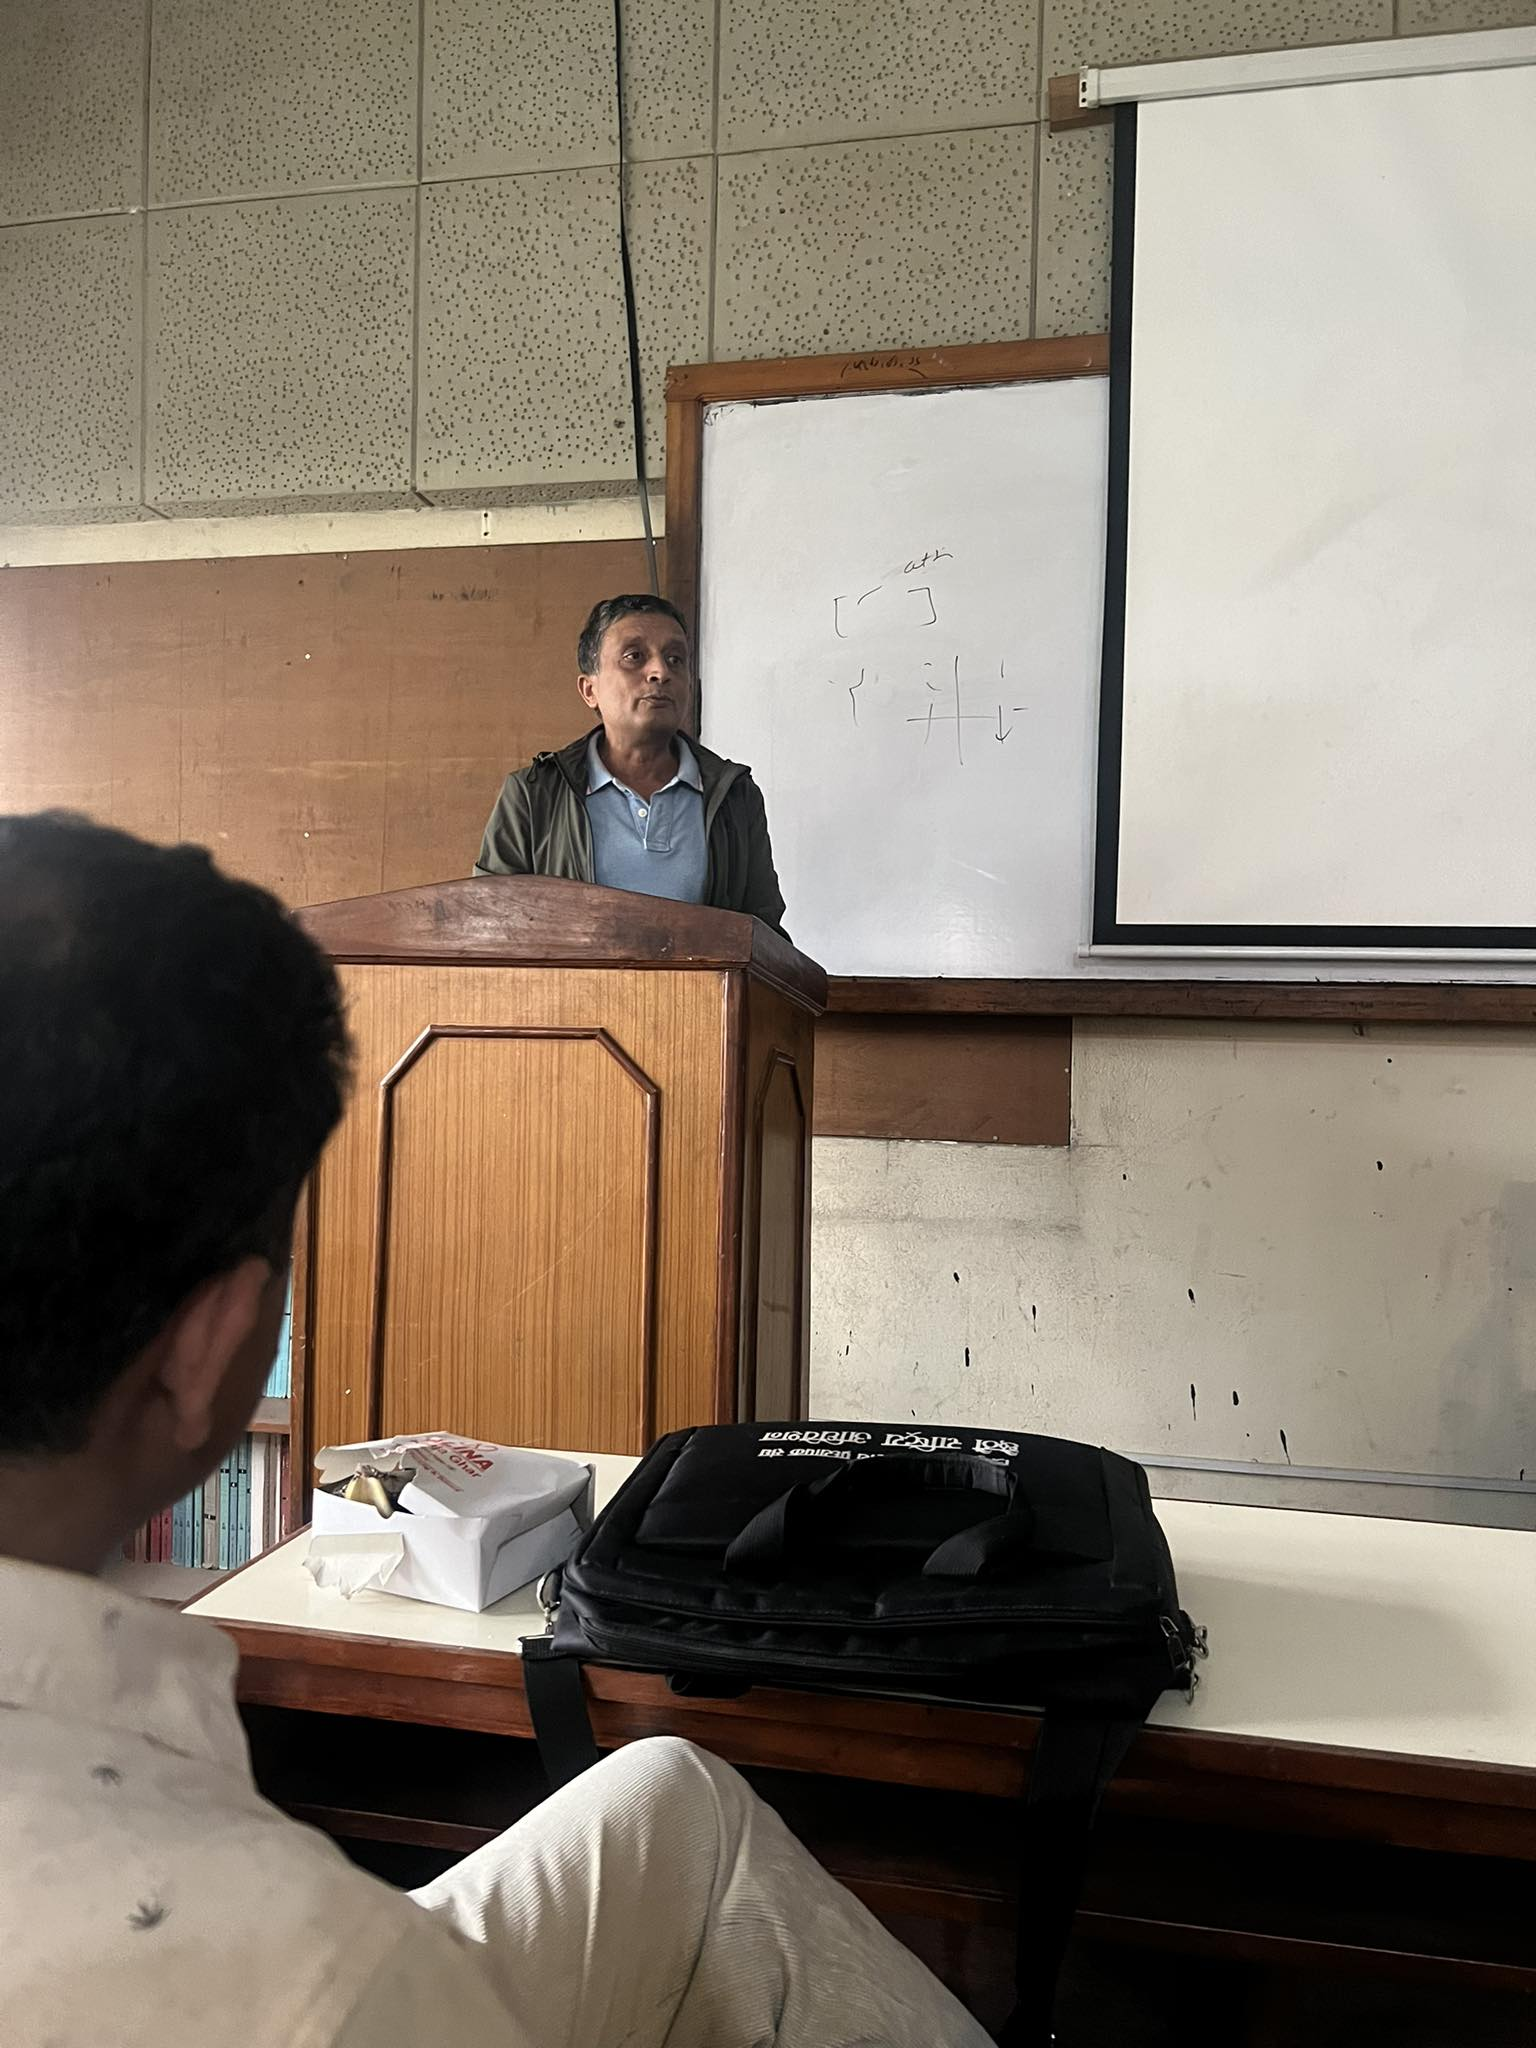
\includegraphics[height=7cm, width=\textwidth]{pramesh.jpg}
  \caption{Dr. Kattel}
\end{subfigure}
\hfill
\begin{subfigure}{0.45\textwidth}
  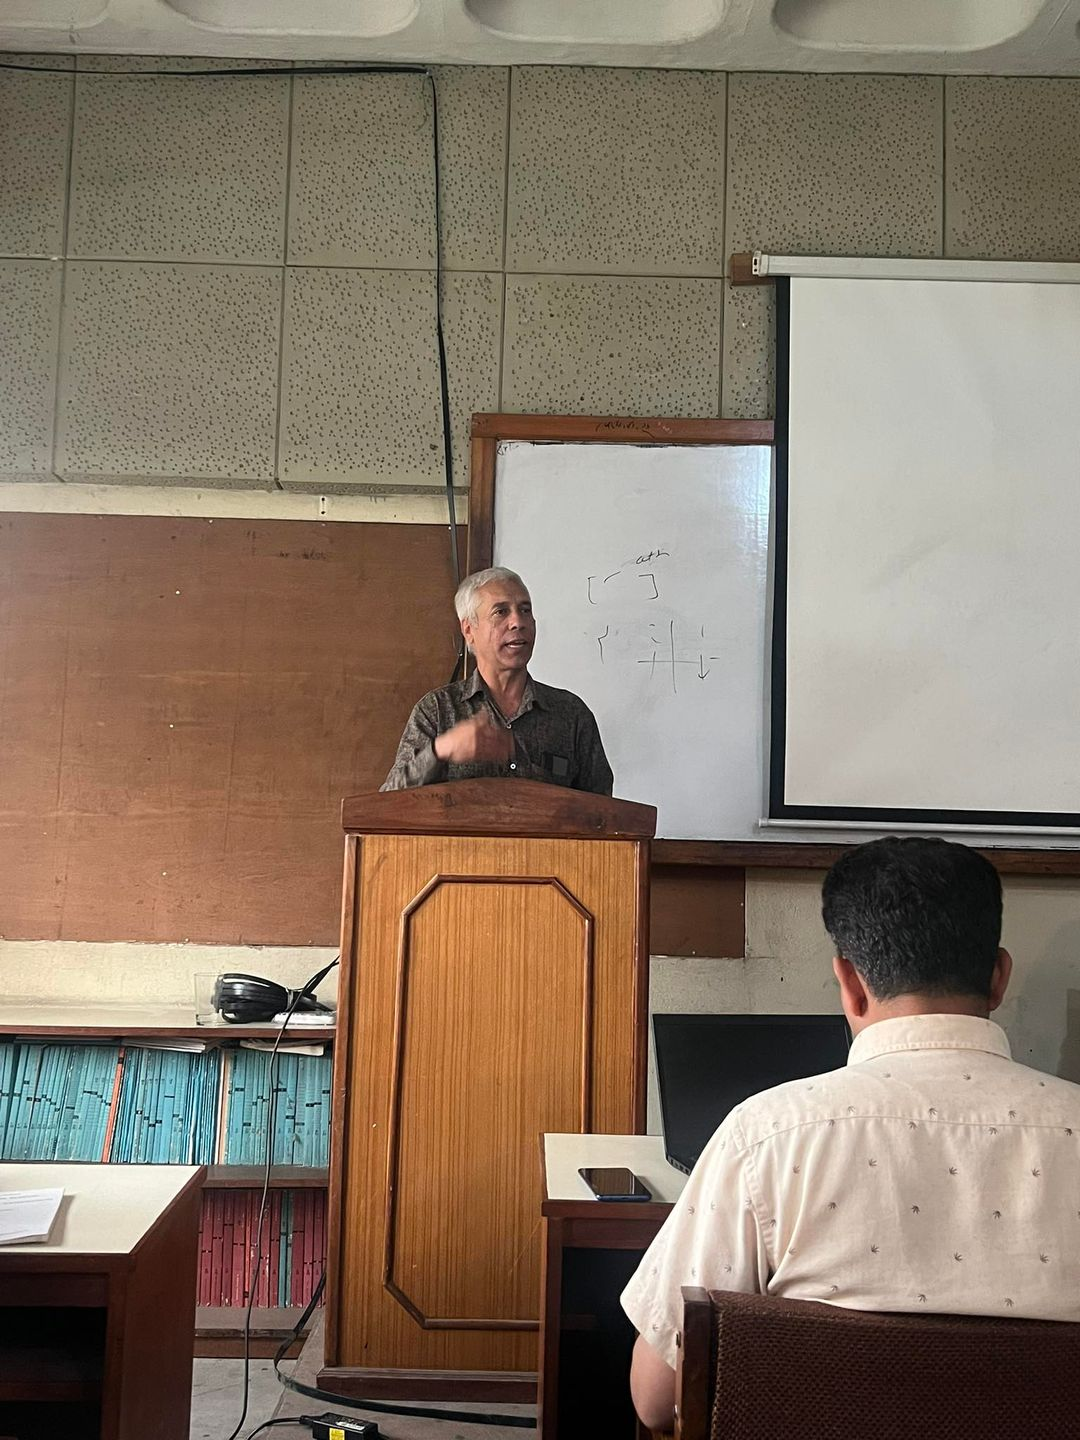
\includegraphics[height=7cm, width=\textwidth]{dinesh.jpg}
  \caption{Dr. Panthi}
\end{subfigure}
\end{figure}

\vspace{7mm}
Among the guests Dr. Panthi remarked the success of the workshop and suggested the participants to keep practicing the latex to learn it well. Dr. Kafle the host and coordinator remarked that it is not possible to learn and understand everything about the latex in a single workshop. We have seen all the workings of the latex and must keep working on it on our own as well to fully master it. So one should not be dissapointed if there is some concept he/she has not understood it fully. Finally he declared the conclusion of the workshop.
\clearpage

\vspace*{5mm}
{\bfseries \large Token of Love to the Guests}
\vspace{3mm}
\begin{figure}[h!]
\centering
\begin{subfigure}[c]{0.33\textwidth}
  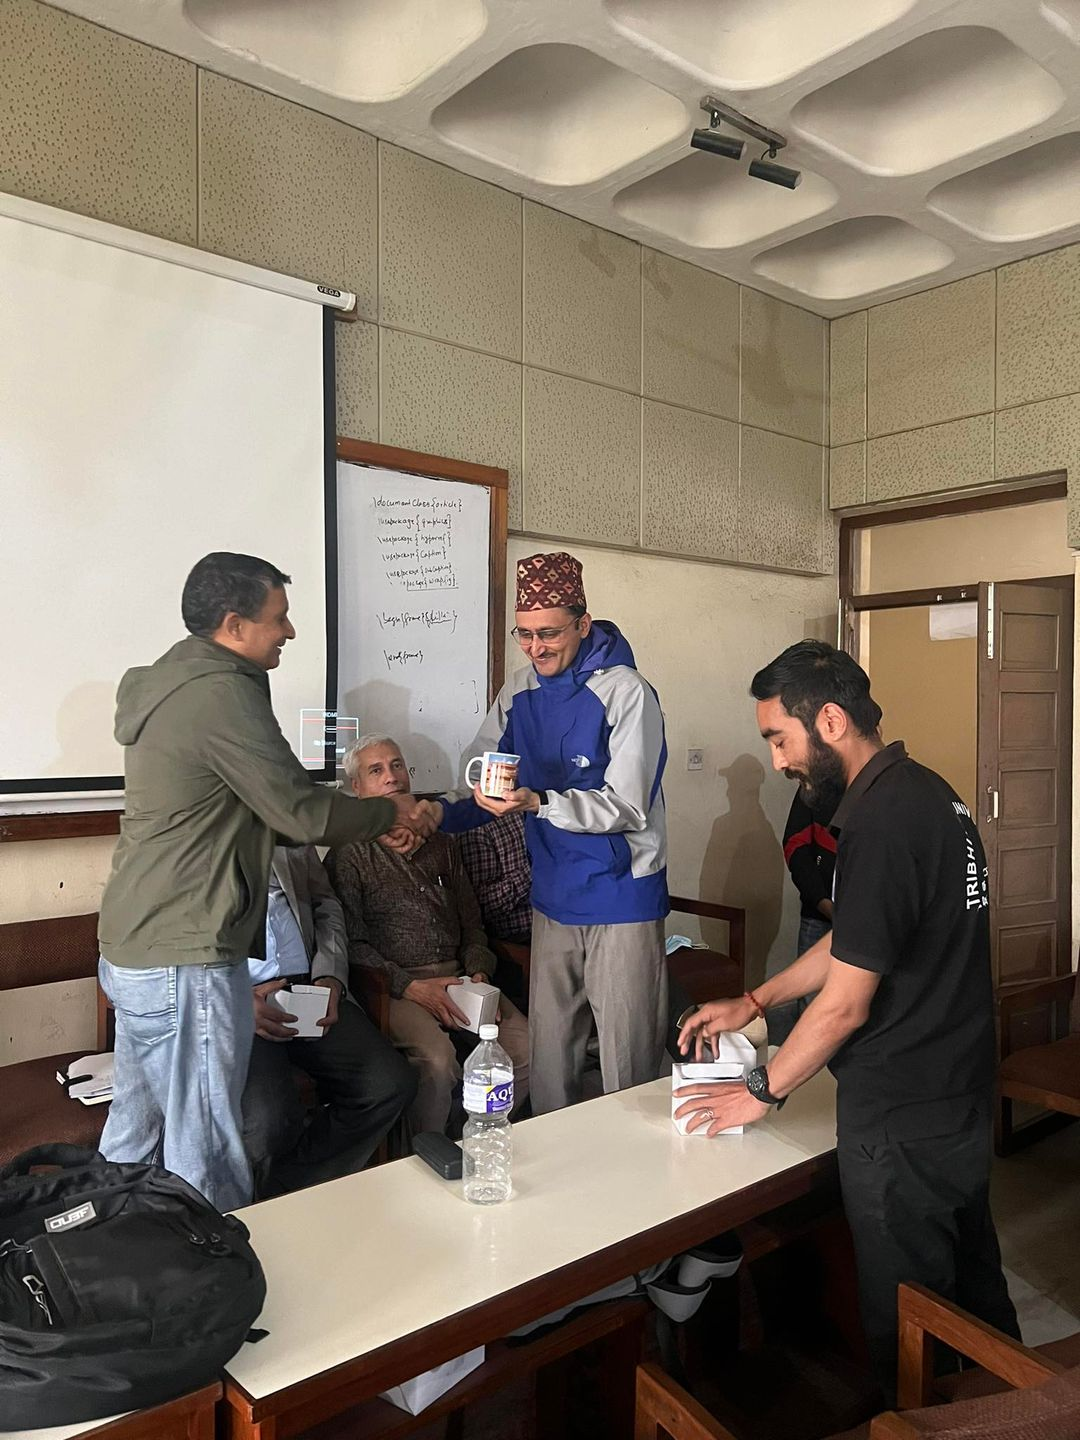
\includegraphics[height=7cm, width=\textwidth]{rcdt.jpg}
  \caption{Dr. Dhungana}
\end{subfigure}
\hfill
\begin{subfigure}[t]{0.33\textwidth}
  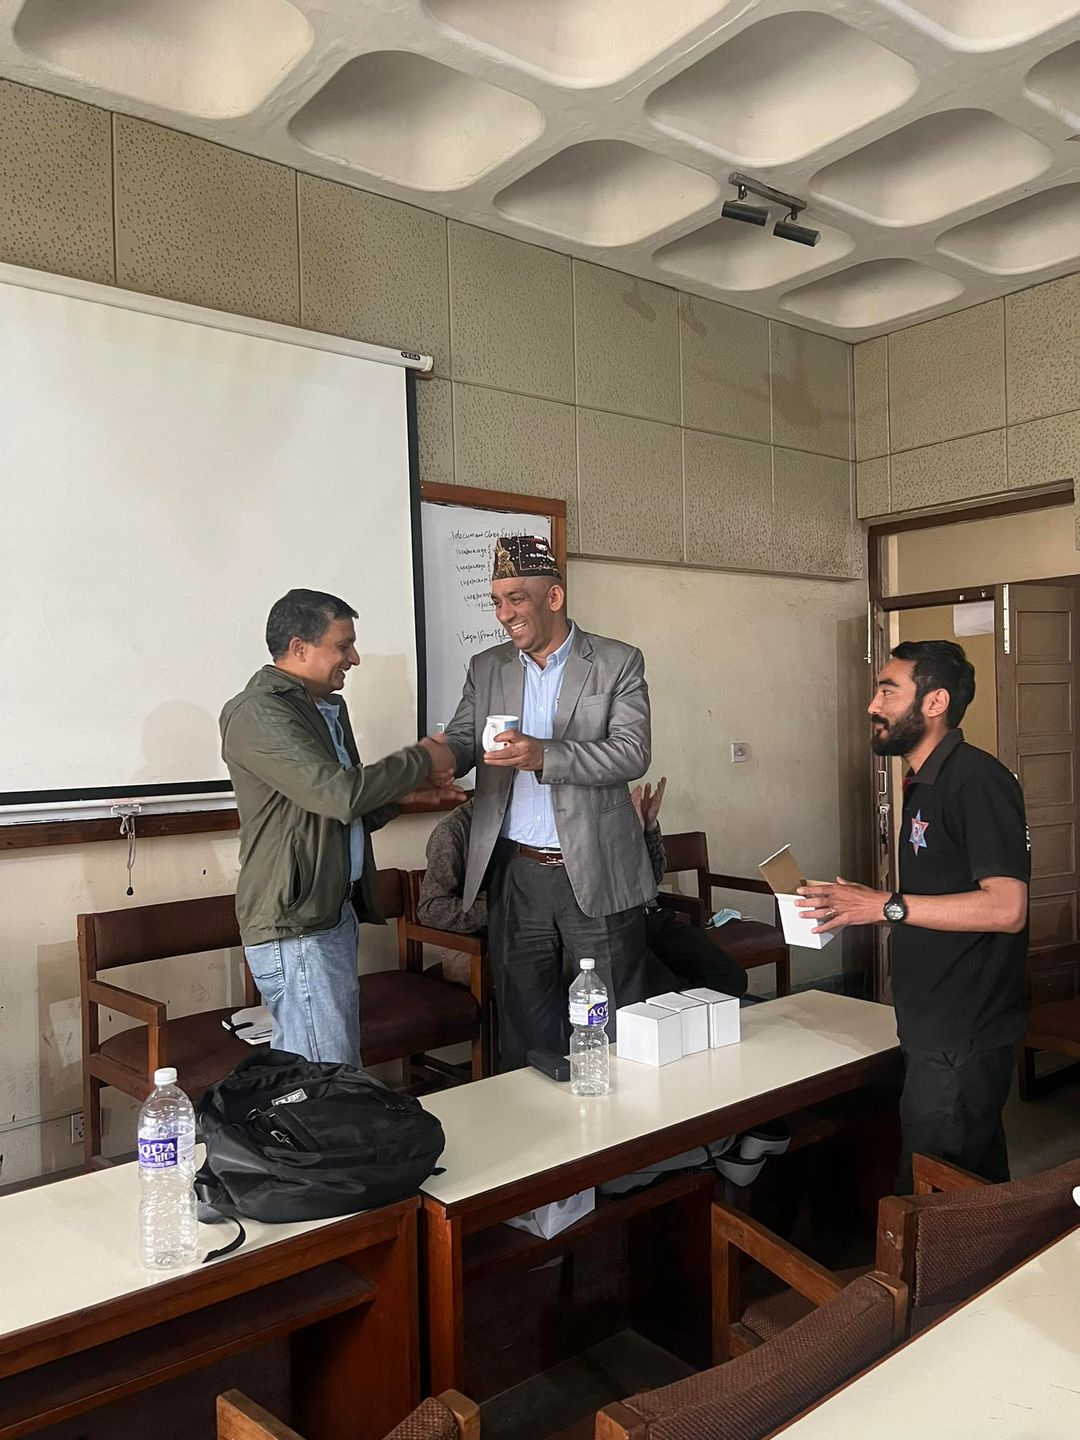
\includegraphics[height=7cm, width=\textwidth]{puskart.jpg}
  \caption{Dr. Pokharel}
\end{subfigure}
\hfill
\begin{subfigure}[b]{0.3\textwidth}
  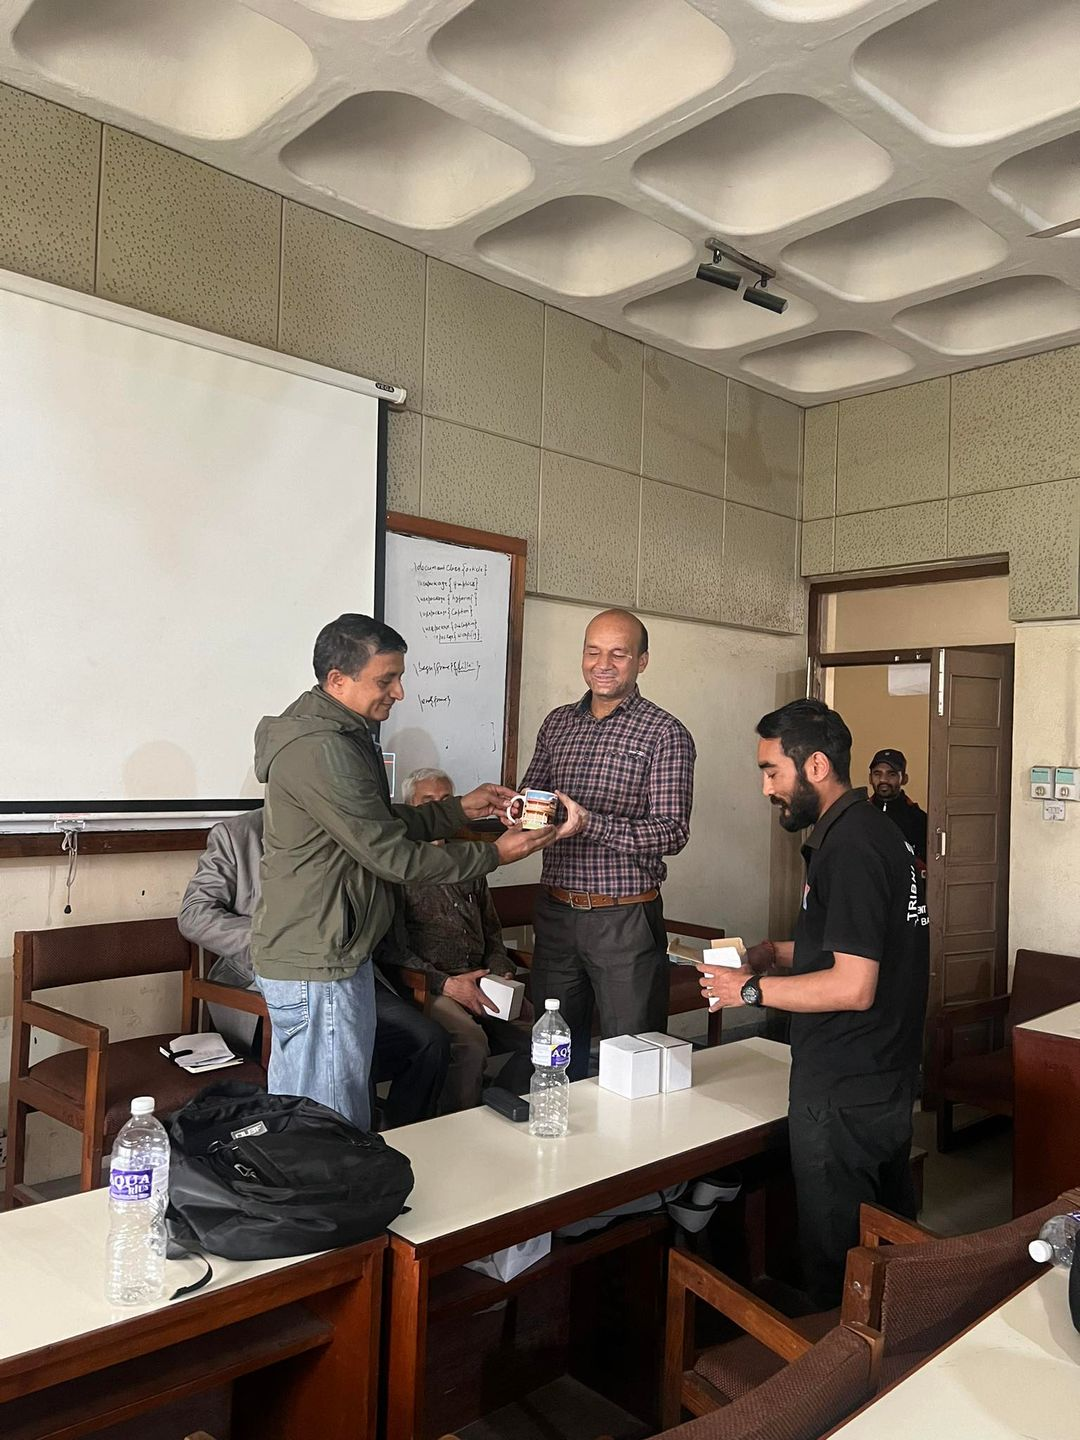
\includegraphics[height=7cm, width=\textwidth]{santosht.jpg}
  \caption{Dr. Ghimire}
\end{subfigure}
\end{figure}


\vspace*{10mm}
{\bfseries \large Certificate Distribution Clips}

\begin{figure}[h!]
\centering
\begin{subfigure}{0.32\textwidth}
  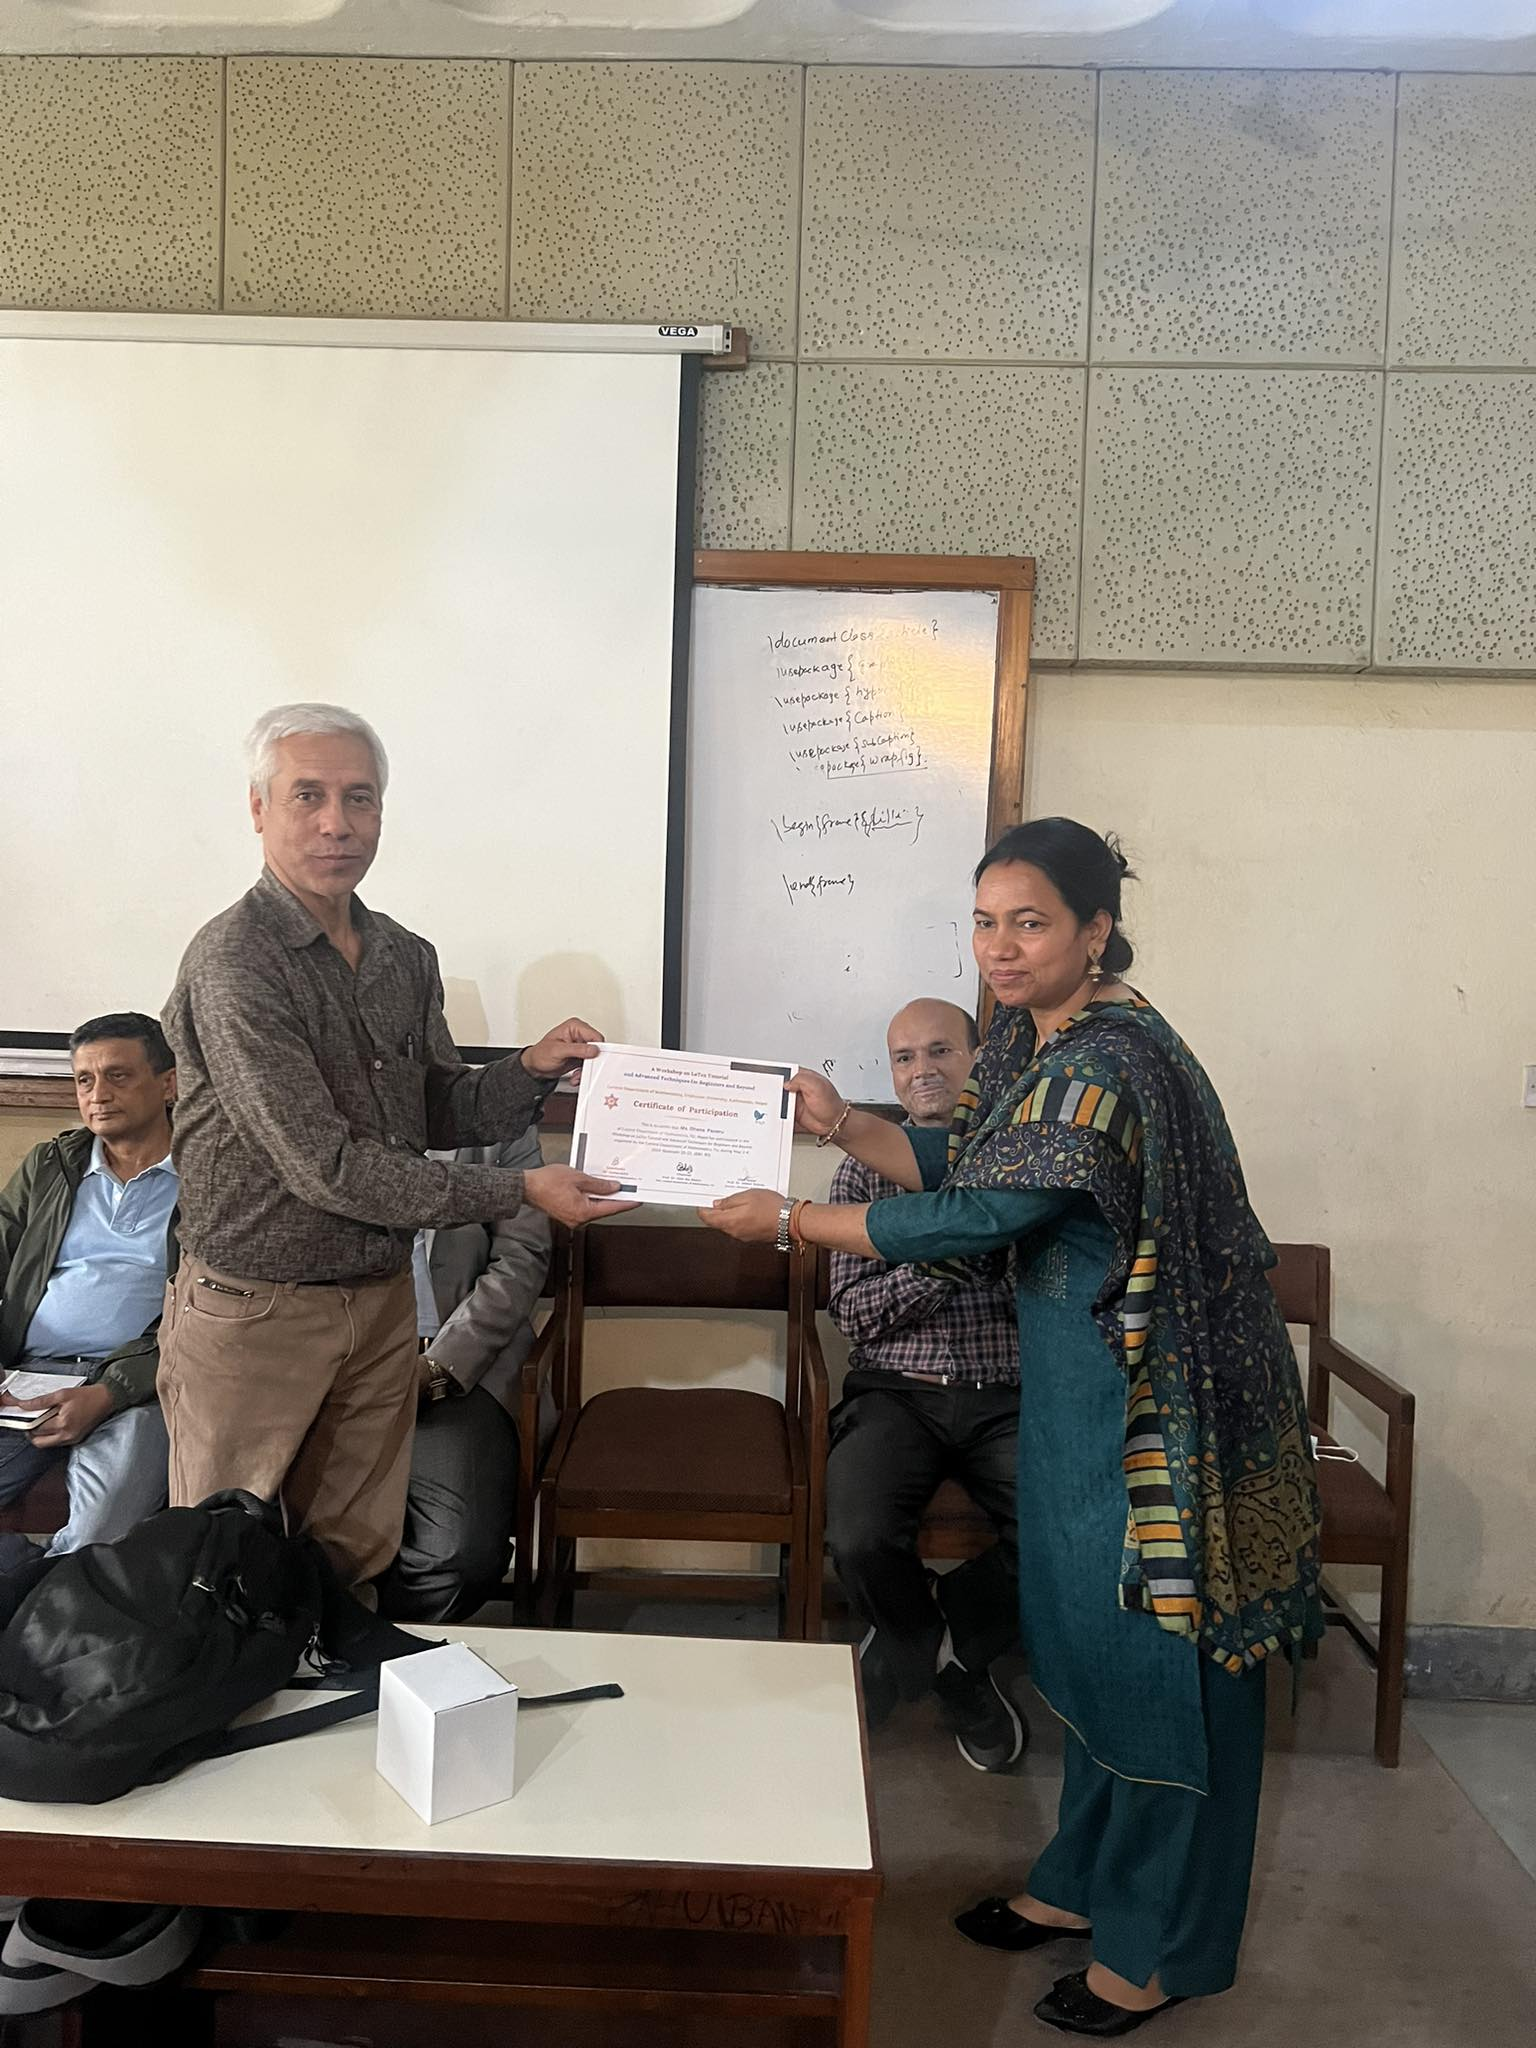
\includegraphics[height=6.5cm, width=\textwidth]{dhanamaam.jpg}
\end{subfigure}
\hfill
\begin{subfigure}{0.31\textwidth}
  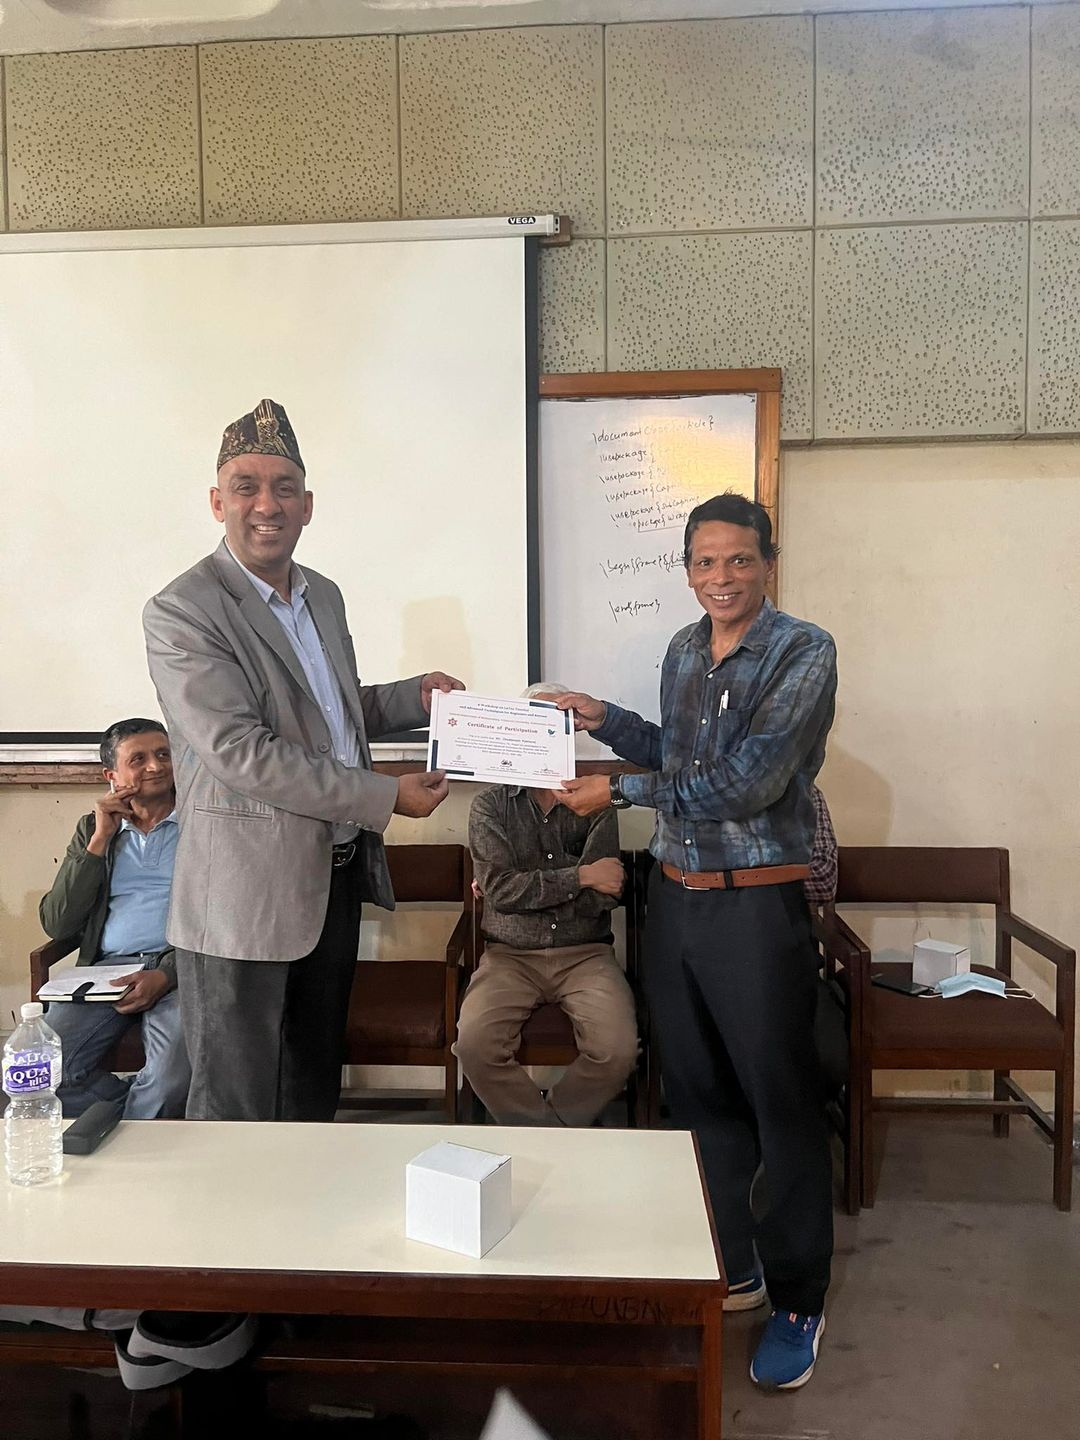
\includegraphics[height=6.5cm, width=\textwidth]{chudamani.jpg}
\end{subfigure}
\hfill
\begin{subfigure}{0.32\textwidth}
  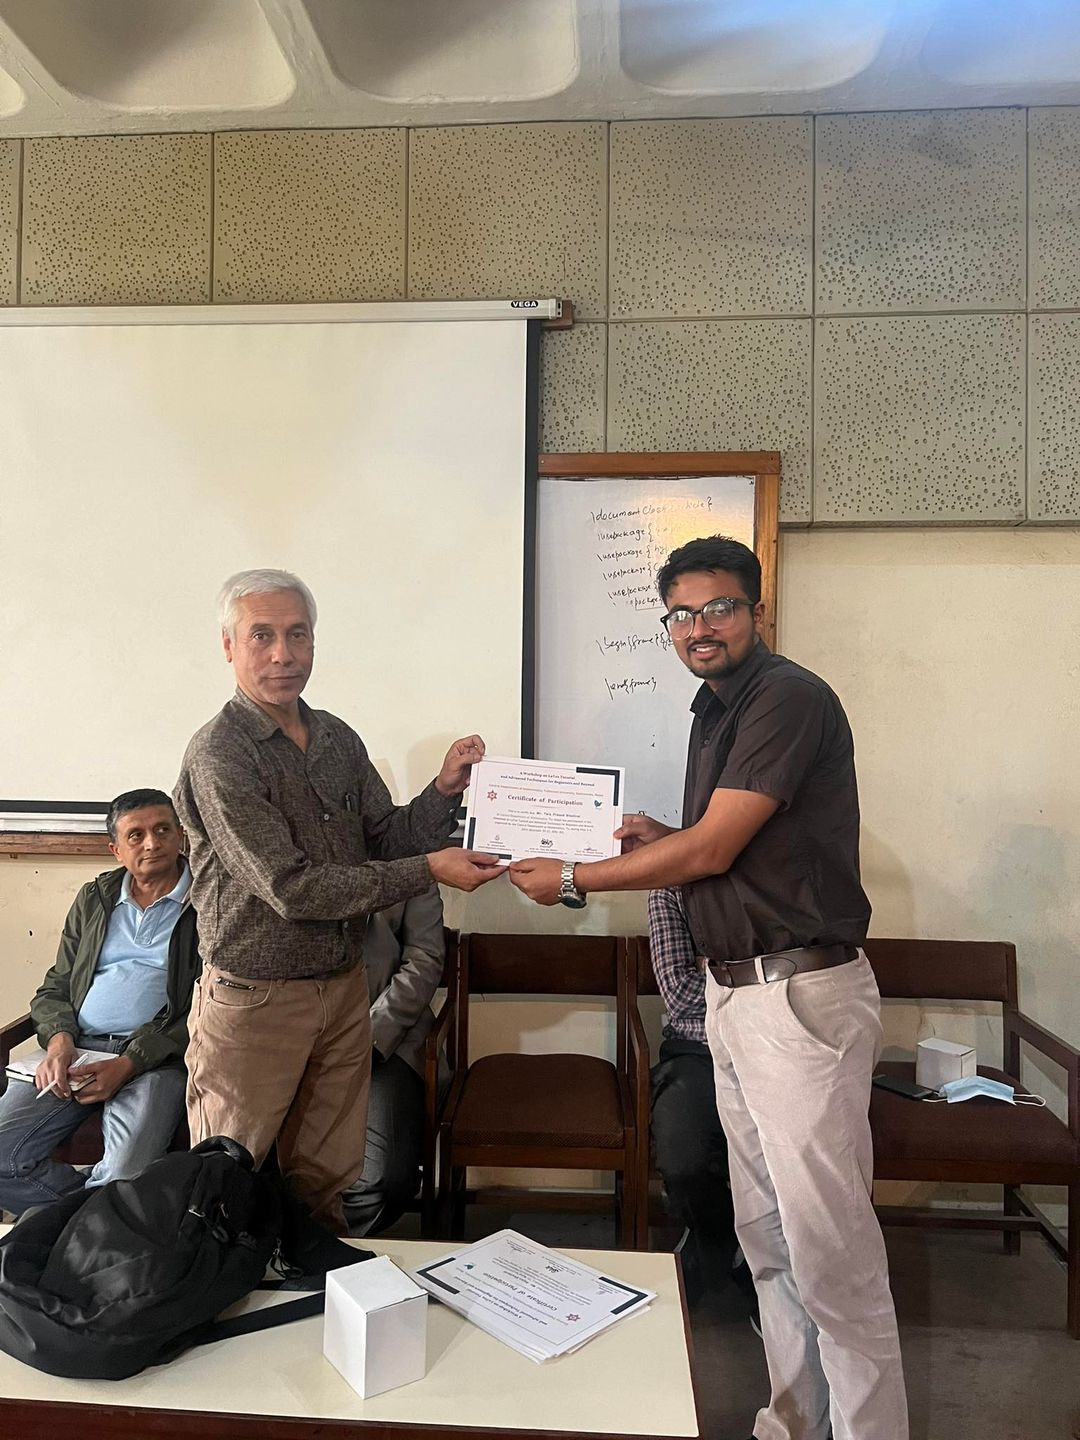
\includegraphics[height=6.5cm, width=\textwidth]{tara.jpg}
\end{subfigure}
\end{figure}

\clearpage

\vspace*{10mm}
{\bfseries \large News}\\[3mm]
The news of the workshop was covered by the \textbf{Nayapaila} media which is an online media: \href{https://nayapailaonline.com/2024/05/08/%e0%a4%97%e0%a4%a3%e0%a4%bf%e0%a4%a4-%e0%a4%95%e0%a5%87%e0%a4%a8%e0%a5%8d%e0%a4%a6%e0%a5%8d%e0%a4%b0%e0%a5%80%e0%a4%af-%e0%a4%b5%e0%a4%bf%e0%a4%ad%e0%a4%be%e0%a4%97%e0%a4%ae%e0%a4%be-%e0%a5%a9/}{News Link}.


\vspace*{50mm}

{\bfseries \large Group Photo at the end}
\vspace*{5mm}

\begin{figure}[h!]
  \centering
  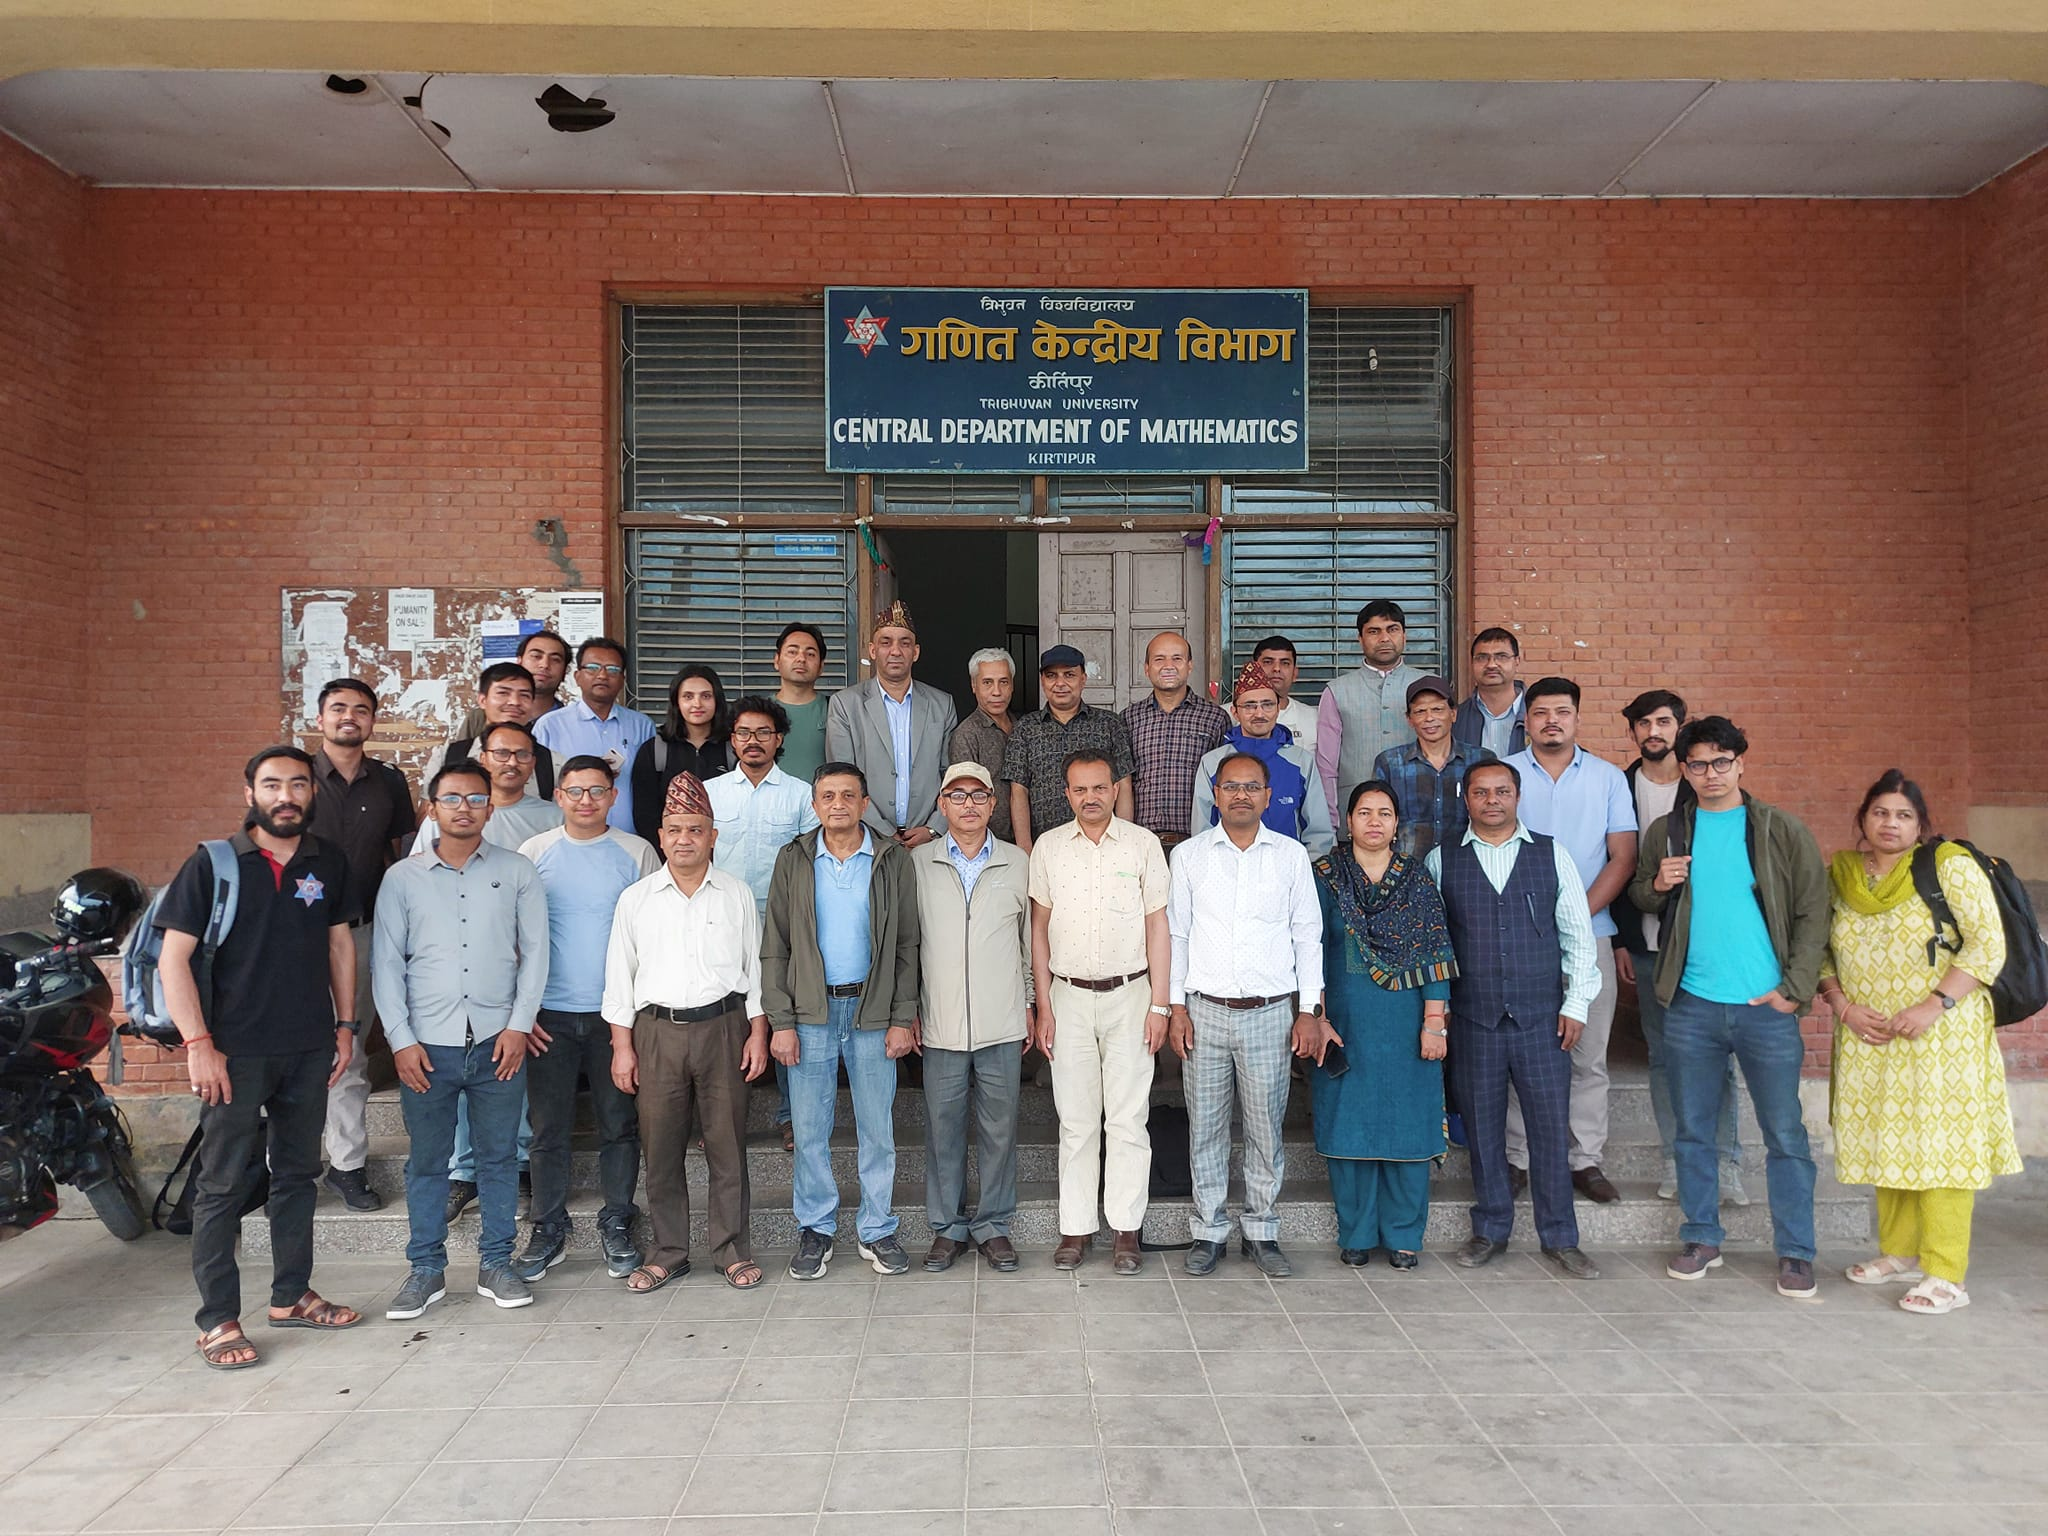
\includegraphics[width=15cm, height=11cm]{group.jpg}
\end{figure}
\clearpage

\vspace*{2cm}
{\bfseries \Large Outputs}\\[5mm]
Following were the outputs of the workshop.

\begin{enumerate}
\item Good collaboration between the faculties of various campuses and the students.
\item Participants were literate on latex at both basic and advance level.
\item Participants were able to write an article, a report and make a
  presentation in latex at the end.
  \item Participants also learned computer skills as a side skill while learning latex.
\end{enumerate}

\vspace{4cm}
{\bfseries \Large Conclusions and Recommendations} \vspace{1mm}
\begin{enumerate}
\item Such workshops are very helpful in both teaching and learning, and sharing new knowledge.
\item For a skill like latex workshop are the best mode of learning.
\item Workshops on such as latex should be at least of few days. More the days the better.
\item Such workshops should be coordinated and conducted from time to time at least once a month.
  \item Some budget and resources should be allocated for the workshops also.
\end{enumerate}

\clearpage

{\bfseries \large List of registered Participants}
\begin{figure}[h!]
  \centering
  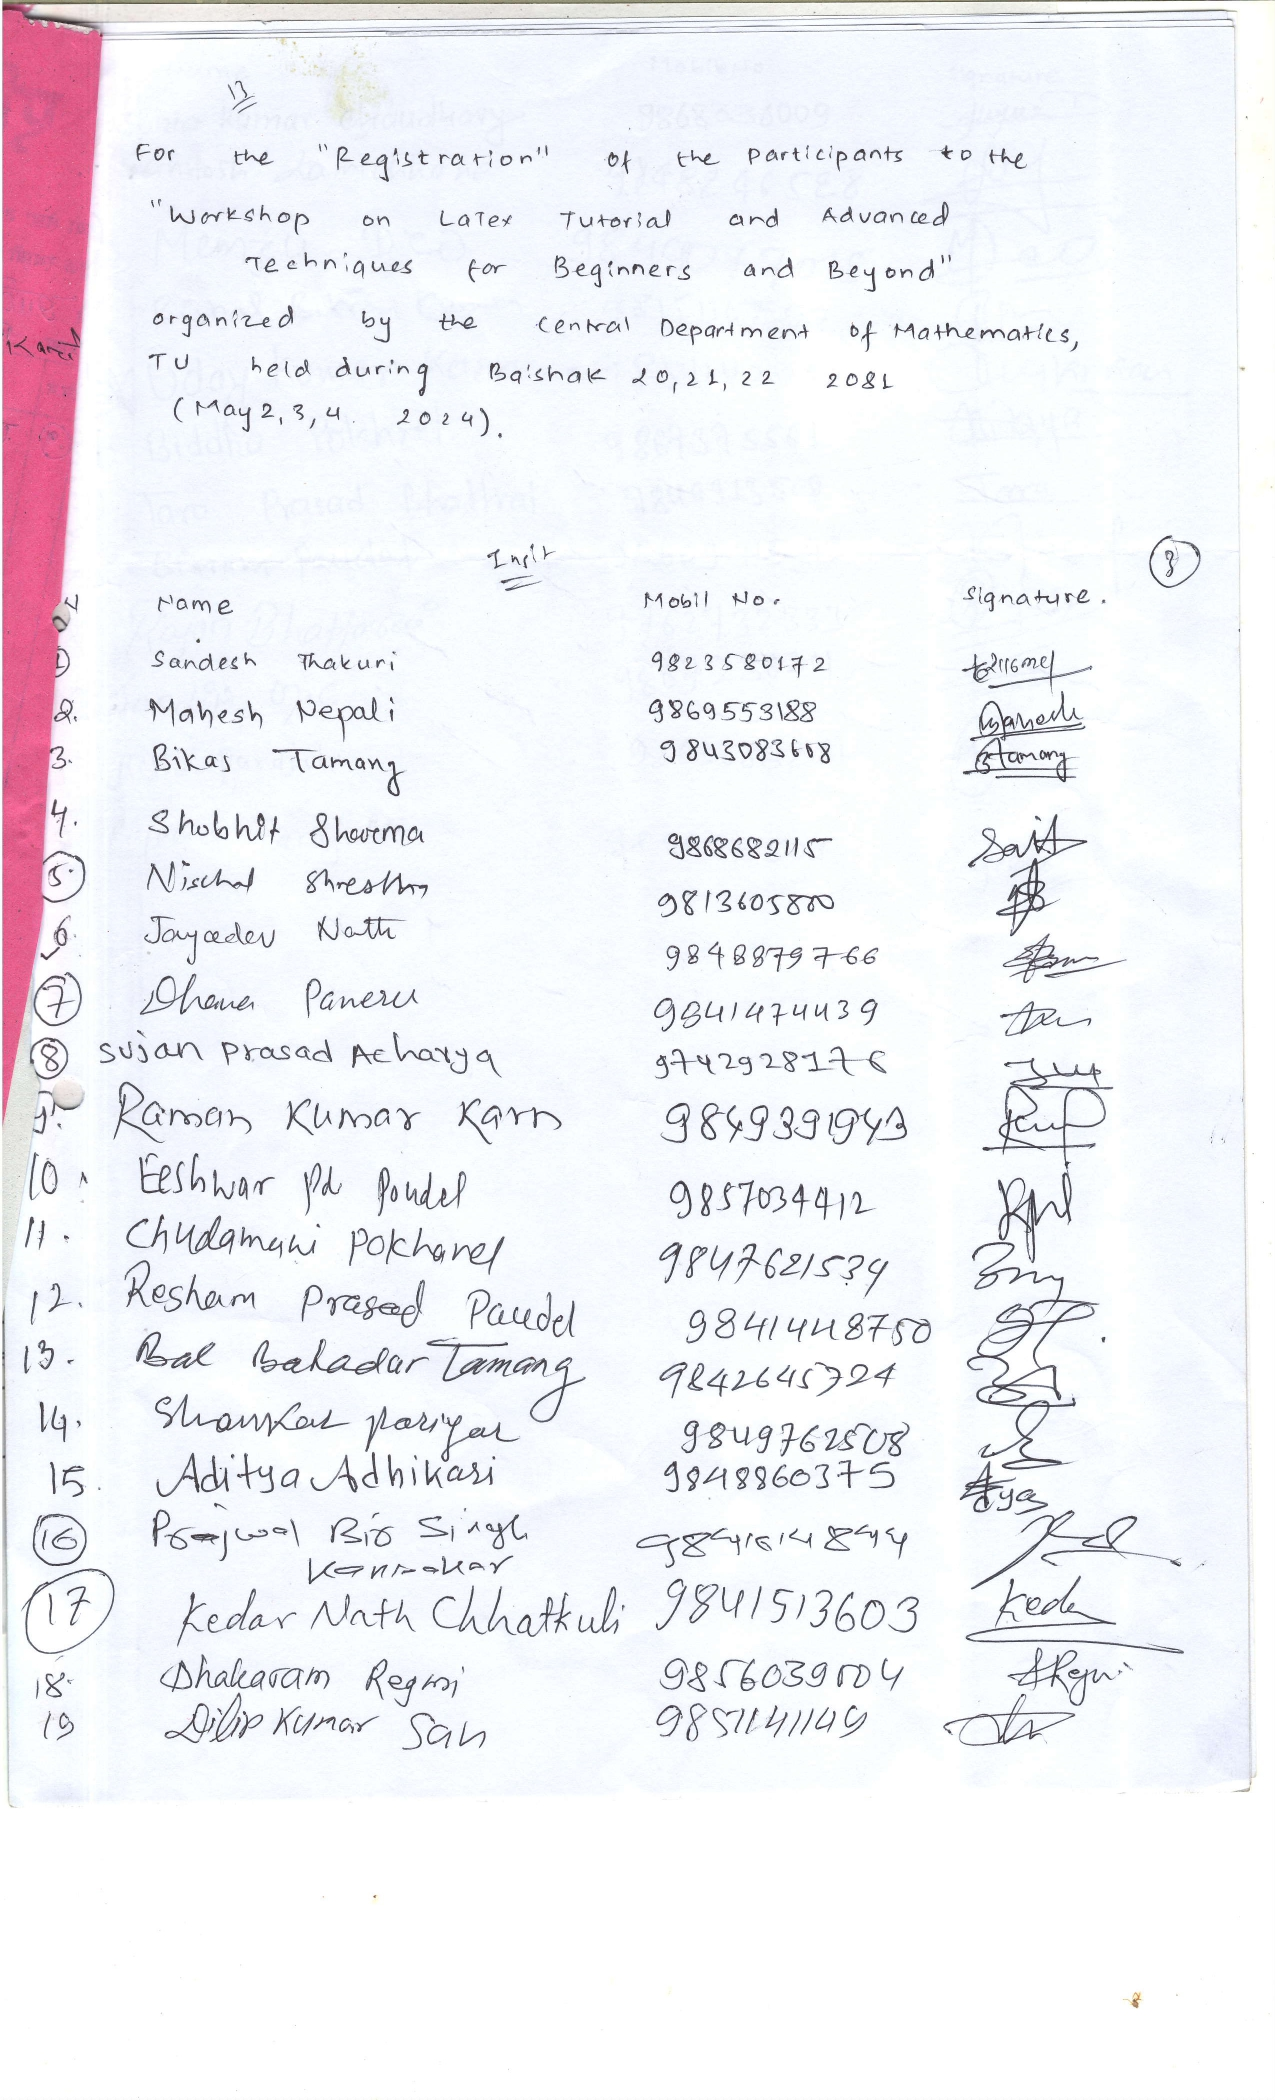
\includegraphics[width=12cm, height=15cm]{scan1.jpg}
  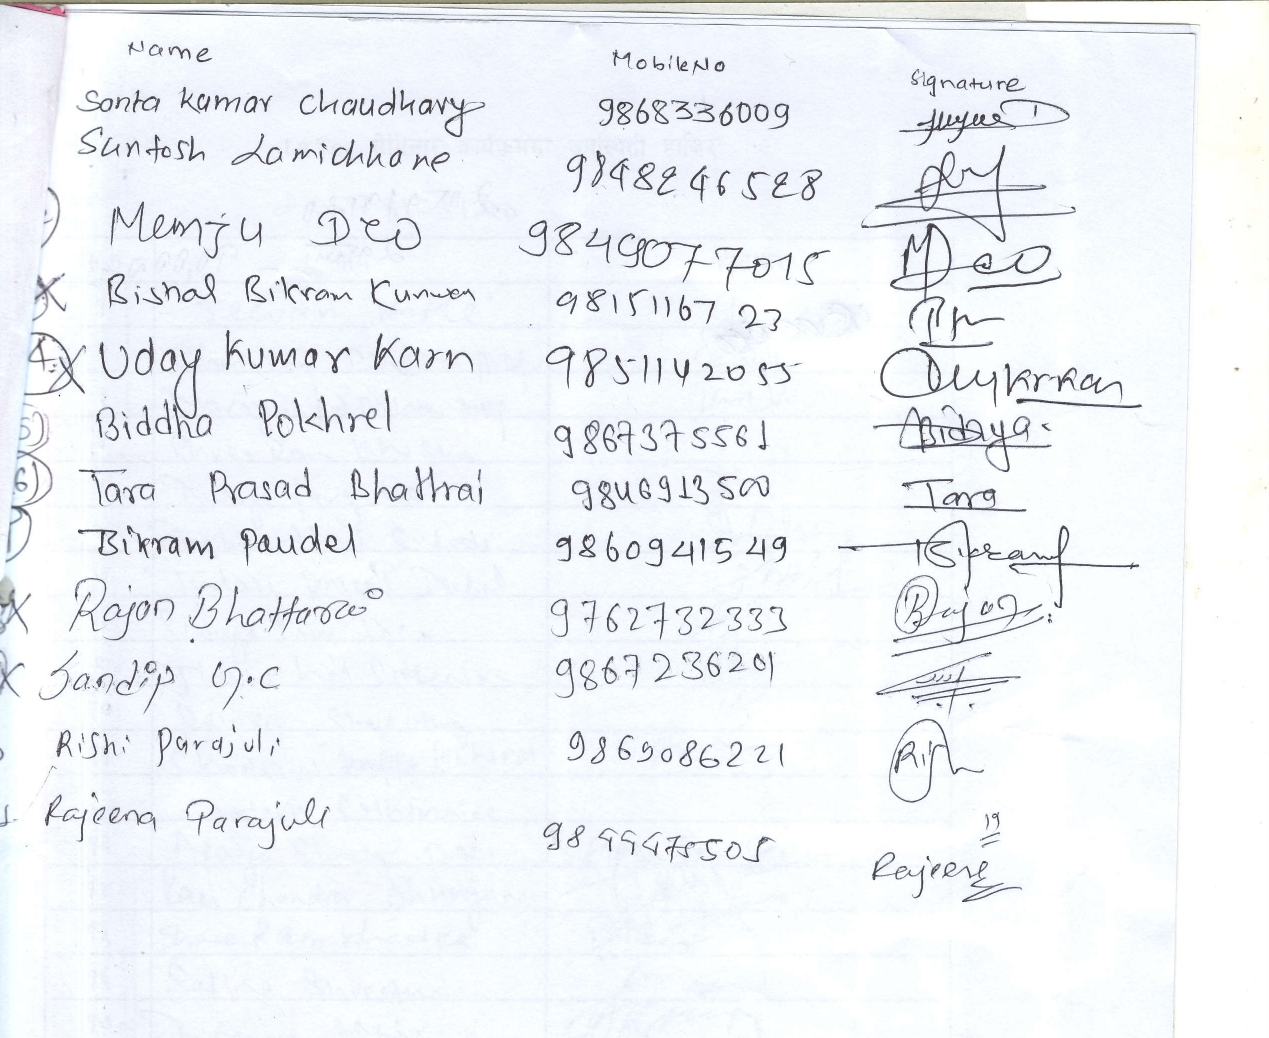
\includegraphics[width=12cm, height=10cm]{scan2.jpg}
\end{figure}

\end{document}
%%% Local Variables:
%%% mode: latex
%%% TeX-master: t
%%% End:
